\chapter{\ifproject%
\ifenglish Project Structure and Methodology\else โครงสร้างและขั้นตอนการทำงาน\fi
\else%
\ifenglish Project Structure\else โครงสร้างของโครงงาน\fi
\fi
}

ในบทนี้จะกล่าวถึงหลักการ และการออกแบบระบบ

\makeatletter

% \renewcommand\section{\@startsection {section}{1}{\z@}%
%                                    {13.5ex \@plus -1ex \@minus -.2ex}%
%                                    {2.3ex \@plus.2ex}%
%                                    {\normalfont\large\bfseries}}

\makeatother
%\vspace{2ex}
% \titleformat{\section}{\normalfont\bfseries}{\thesection}{1em}{}
% \titlespacing*{\section}{0pt}{10ex}{0pt}

\section{เนื้อหา}

\subsection{เนื้อเรื่อง}

เกมนี้มีเนื่อเรื่องและสถานที่อยู่ในยุโรปยุคกลาง ตามความเชื่อที่ว่า ปีศาจสามารถปลอมแปลงเป็นสัตว์ชนิด
หนึ่ง อาศัยอยู่ในป่ารกร้าง หน้าที่ของผู้เล่นคือ ต้องไปปราบปีศาจร้ายและทําให้ผู้คนปลอดภัย

\subsection{ดนตรีและเสียงประกอบ}

เกมนี้มีเสียงประกอบที่สร้างความสมจริงและความสยองขวัญ โดยมีเสียงประกอบทั้งหมด 2 ชนิด ได้แก่ ดนตรี ซาวด์เอฟเฟค
\begin{itemize}
  \item เสียงดนตรี: ถูกเล่นเมื่อผู้เล่นเห็นฝั่งตรงข้ามหรือโจมตีกัน โดยเป็นเสียงดนตรีที่สร้างความระทึก และหยุดเล่นเมื่อผู้เล่นหลบหนีไปห่างจากฝั่งตรงข้าม
  \item เสียงซาวด์เอฟเฟค: ถูกเล่นเมื่อผู้เล่นทำการกระทำต่าง ๆ
\end{itemize}

เสียงซาวด์เอฟเฟคเป็นเสียงแบบ 3 มิติที่มีระยะการได้ยินที่เหมาะสม ซึ่งทำให้ผู้เล่นสามารถระบุตำแหน่งของผู้เล่นคนอื่น ๆ ได้ 
นอกจากนี้แล้วเสียงซาวน์เอฟเฟคการเดินและวิ่งจะขึ้นอยู่กับพื้นผิวที่ผู้เล่นกำลังเคลื่อนที่อยู่เพื่อความสมจริง

\subsection{ฉาก}

สถานที่ของเกมคือป่าสนแห้งแล้งแห่งหนึ่งในยุโรป ดังแสดงในรูปที่ ~\ref{fig:Map} และ ~\ref{fig:atmosphere}  ขนาดของแผนที่ คือ 400 x 400 เมตร ประกอบไปด้วยทะเลสาบ 
น้ำตก ลำธาร ป่าสน และเนินเขา รวมถึงมีบ้านเก่า ๆ ที่ถูกทิ้งไว้ ซึ่งสามารถเป็นจุดนัดพบได้ เวลาของเกมคือช่วงกลางคืน 
สถานที่นอกจากมืดแล้วยังมีหมอกหนา ทำให้มองเห็นได้ไม่ชัดเจน เพื่อเพิ่มความระทึกให้กับผู้เล่น

\begin{figure}[p]
  \begin{center}
  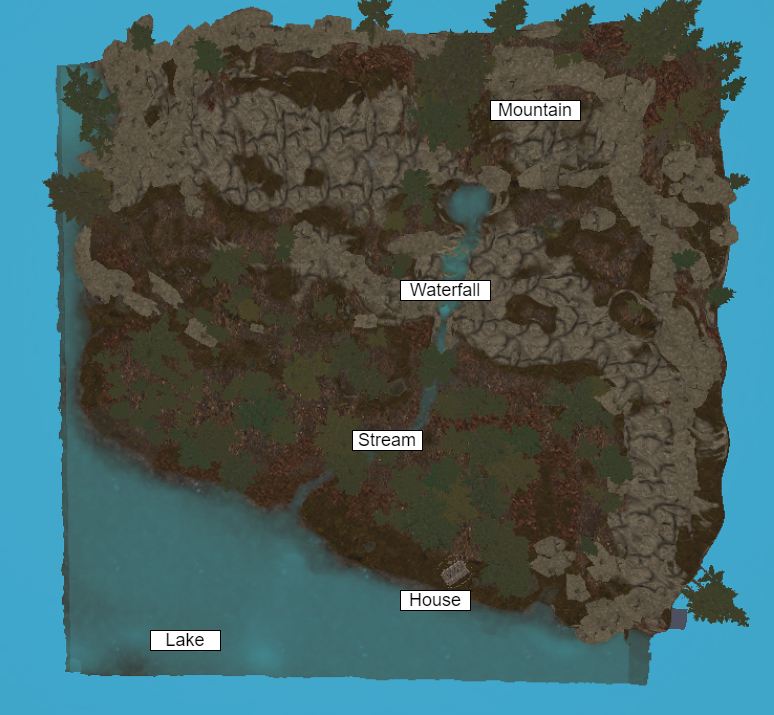
\includegraphics[width=0.7\textwidth]{./img/scene/WitchHunter-Map.png}
  \end{center}
  \caption[ภาพมุมสูงแสดงตำแหน่งของสถานที่ต่าง ๆ
  และภูมิประเทศของฉากในเกม]{ภาพมุมสูงแสดงตำแหน่งของสถานที่ต่าง ๆ
  และภูมิประเทศของฉากในเกม}
  \label{fig:Map}
\end{figure}

\begin{figure}[p]
  \begin{center}
  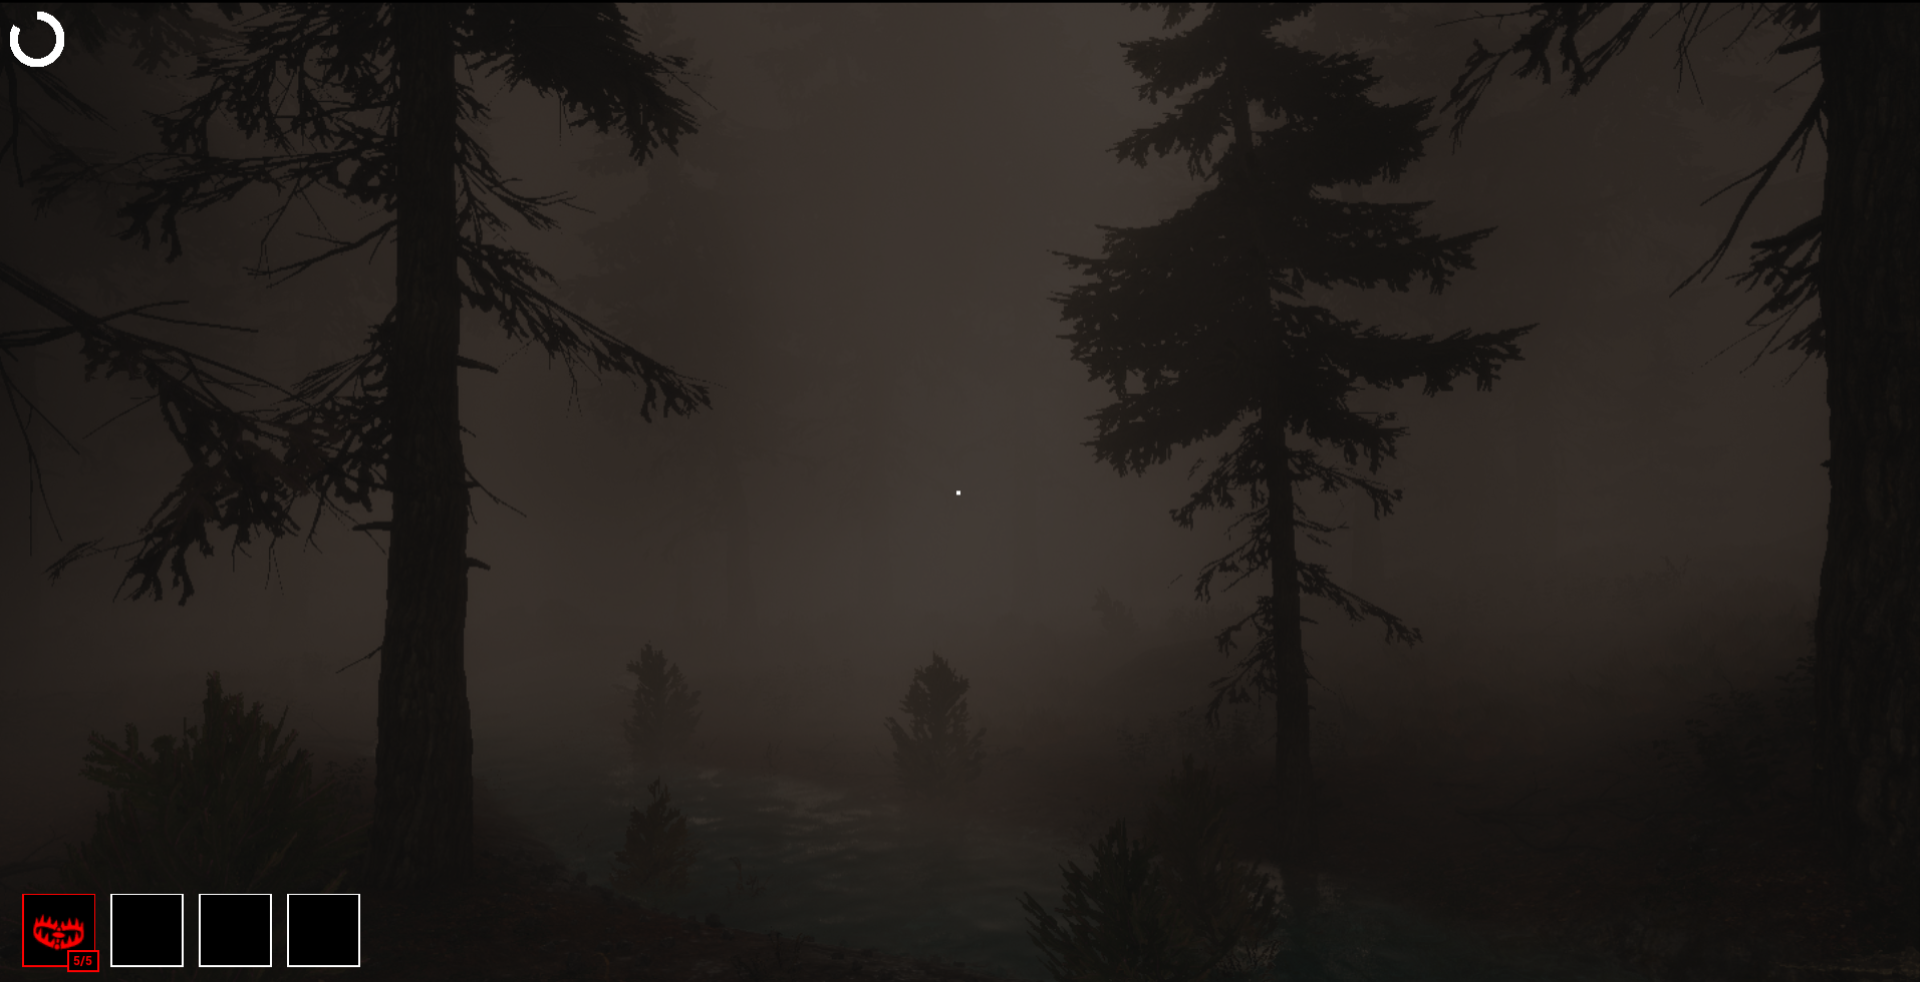
\includegraphics[width=\textwidth]{./img/scene/atmosphere.png}
  \end{center}
  \caption[ภาพบรรยากาศภายในเกม]{ภาพบรรยากาศภายในเกม}
  \label{fig:atmosphere}
\end{figure}

\subsection{ตัวละคร}

ในเกมนี้มีตัวละครทั้งหมด 3 ตัว ได้แก่ 2 ตัวของฝ่าย Hunters และ 1 ตัวของฝ่าย Witch ตัวละครถูกสร้างขึ้นโดยดัดแปลงจากโมเดลเสื้อผ้าและร่างกายที่มีอยู่แล้วในโปรแกรม Reallusion Character Creator

\subsubsection{ตัวละครฝ่าย Hunters}

แบ่งเป็น 2 ตัวละคร ชายและหญิง ซึ่งเป็นนายพรานและมีความสามารถเหมือนกันทั้งคู่ ดังแสดงในรูปที่ ~\ref{fig:emma} และ ~\ref{fig:eric}

\begin{figure}
  \centering
  \begin{subcaptionblock}{.4\textwidth}
    \centering
    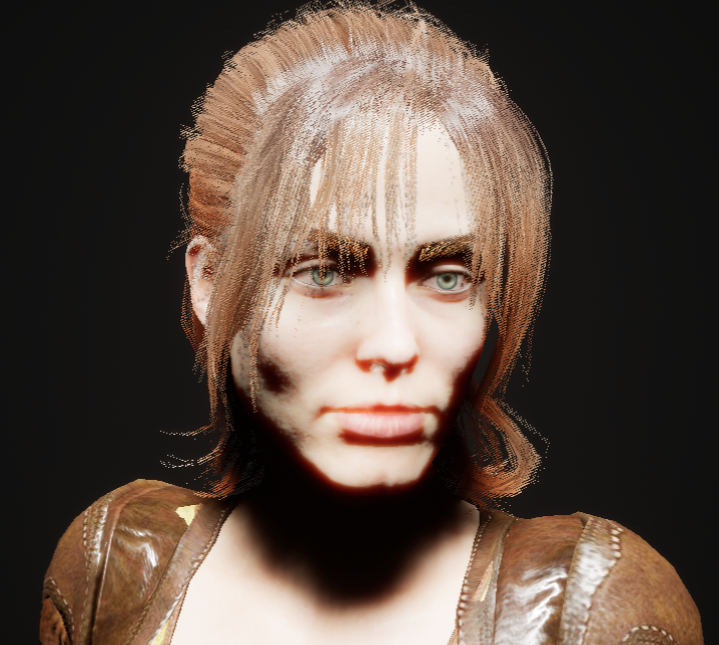
\includegraphics[width=.8\linewidth]{./img/characters/emma_face.png}
    \caption{ภาพใบหน้าตัวละคร Hunter หญิง}\label{ภาพใบหน้าตัวละคร Hunter หญิง}
  \end{subcaptionblock}%
  \begin{subcaptionblock}{.4\textwidth}
    \centering
    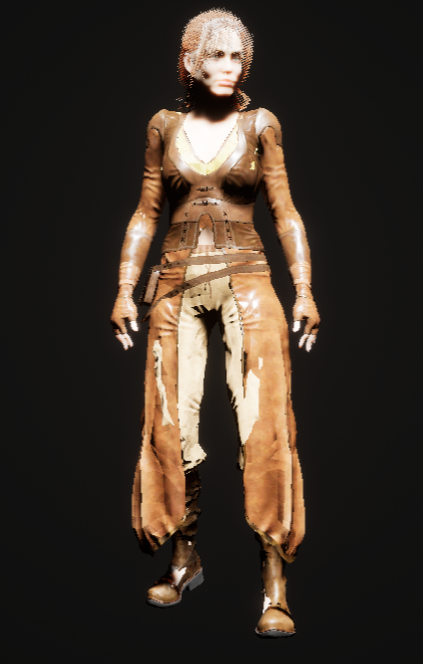
\includegraphics[width=.8\linewidth]{./img/characters/emma_full.png}
    \caption{ภาพเต็มตัวตัวละคร Hunter หญิง}\label{ภาพตัวเต็มตัวละคร Hunter หญิง}
  \end{subcaptionblock}%
  \caption{ภาพตัวละคร Hunter หญิง}\label{fig:emma}
\end{figure}

\begin{figure}
  \centering
  \begin{subcaptionblock}{.4\textwidth}
    \centering
    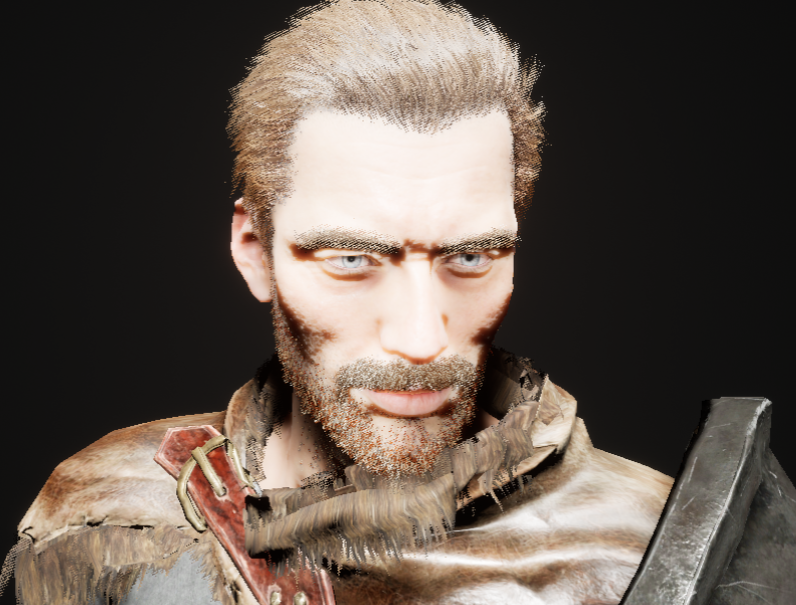
\includegraphics[width=.8\linewidth]{./img/characters/eric_face.png}
    \caption{ภาพใบหน้าตัวละคร Hunter ชาย}\label{ภาพใบหน้าตัวละคร Hunter ชาย}
  \end{subcaptionblock}%
  \begin{subcaptionblock}{.4\textwidth}
    \centering
    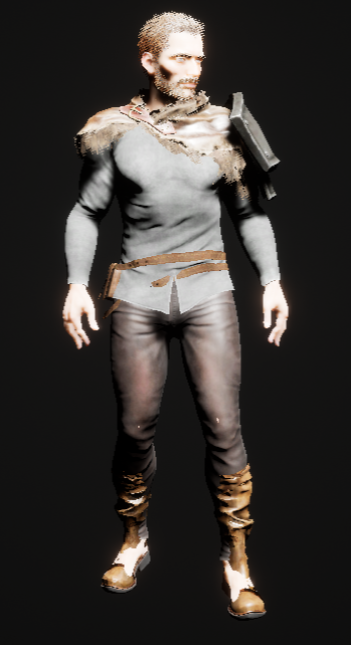
\includegraphics[width=.8\linewidth]{./img/characters/eric_full.png}
    \caption{ภาพเต็มตัวตัวละคร Hunter ชาย}\label{ภาพตัวเต็มตัวละคร Hunter ชาย}
  \end{subcaptionblock}%
  \caption{ภาพตัวละคร Hunter ชาย}\label{fig:eric}
\end{figure}

\subsubsection{ตัวละครฝ่าย Witch}

ร่างของแม่มดจะเป็นหญิงแก่หน้าตาอัปลักษณ์ที่มีศีรษะหันไปด้านหลังและเดินถอยหลัง ดังแสดงในรูปที่ ~\ref{fig:witch}

\begin{figure}
  \centering
  \begin{subcaptionblock}{.4\textwidth}
    \centering
    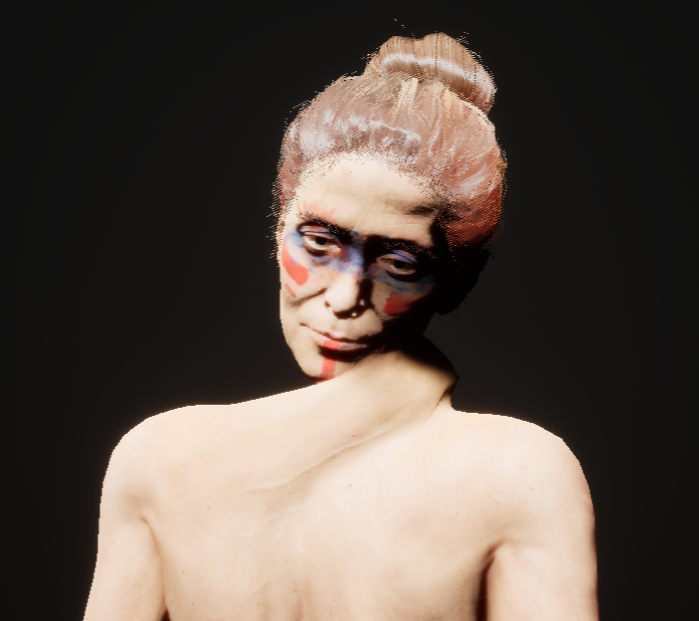
\includegraphics[width=.8\linewidth]{./img/characters/witch_face.png}
    \caption{ภาพใบหน้าตัวละคร Witch}\label{ภาพใบหน้าตัวละคร Witch}
  \end{subcaptionblock}%
  \begin{subcaptionblock}{.4\textwidth}
    \centering
    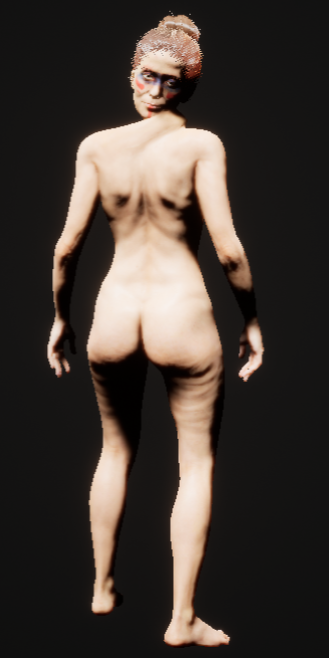
\includegraphics[width=.8\linewidth]{./img/characters/witch_full.png}
    \caption{ภาพเต็มตัวตัวละคร Witch}\label{ภาพตัวเต็มตัวละคร Witch}
  \end{subcaptionblock}%
  \caption{ภาพตัวละคร Witch}\label{fig:witch}
\end{figure}

\begin{figure}[p]
  \begin{center}
  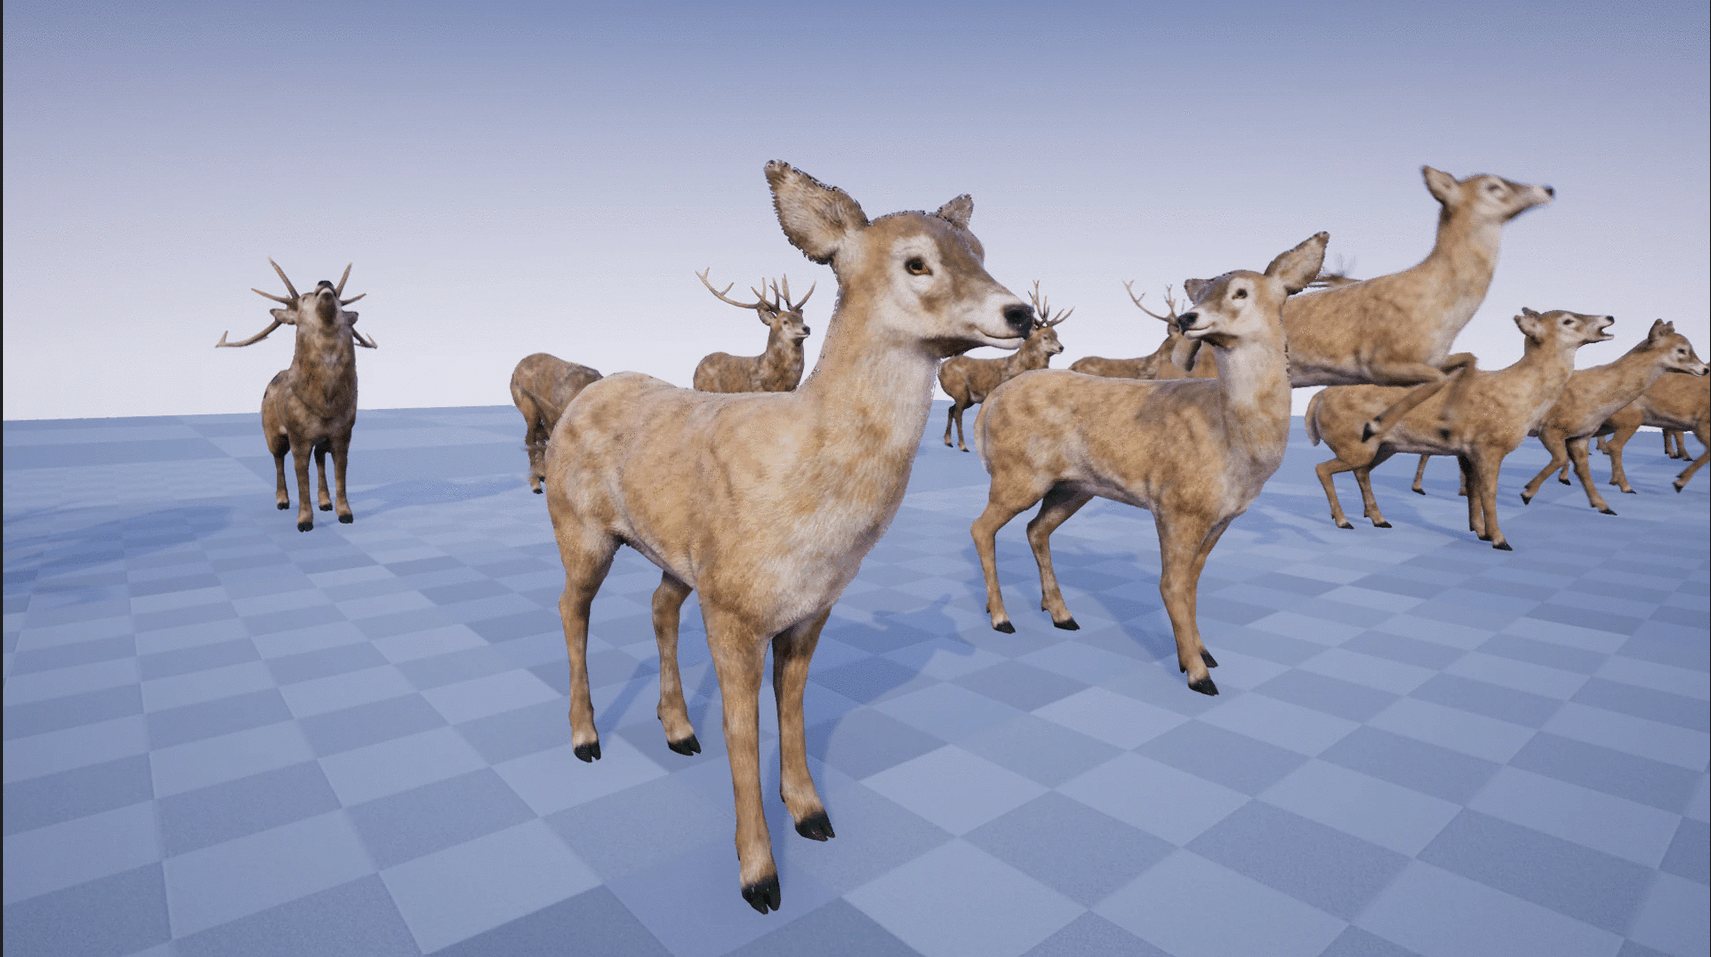
\includegraphics[width=\textwidth]{./img/characters/deerdoe.png}
  \end{center}
  \caption[ภาพตัวละครกวาง]{ภาพตัวละครกวาง}
  \label{fig:deer}
\end{figure}

\subsubsection{ตัวละครกวาง}

กวางสามารถนอน กิน และเดินไปมาได้ อีกทั้งยังสามารถวิ่งหนี Hunter ที่พยายามจับได้อีกด้วย นอกเหนือจากนี้แล้วกวางยังสามารถถูกควบคุมได้โดย Witch เพื่อหลอกล่อ Hunter

\section{วิธีการเล่น}

เพชฌฆาตแม่มด (Witch Hunter) เป็นเกมสยองขวัญแบบหลายผู้เล่น 2vs1 โดยผู้เล่นแบ่งออกเป็น 2 ฝั่ง 
ฝั่งของ Hunters ประกอบด้วยผู้เล่น 2 คน ต้องร่วมมือกันทำภารกิจที่กำหนดไว้ ซึ่งก็คือการจับกวางที่เป็นลูกสมุนของแม่มด 
แล้วนำเลือดกวางมาทำพิธี 6 ครั้งตามจุดที่กำหนดไว้แบบสุ่ม ในขณะที่ฝั่ง Witch ซึ่งประกอบด้วยผู้เล่น 1 คน
ต้องขัดขวางและถ่วงเวลาฝ่าย Hunters ไม่ให้ทำภารกิจสำเร็จ โดยการปลอมตัวเป็นกวางเพื่อหลอกล่อ Hunters และทำการโจมตีด้วยเวทมนต์

\subsection{การเล่นของฝ่าย Hunters}

\subsubsection{การจับกวาง}

สามารถจับกวางด้วยการปามีดศักดิ์สิทธิ์หรือวางกับดักทิ้งไว้ ดังแสดงในรูปที่ ~\ref{fig:การจับกวางโดยใช้มีด} และ ~\ref{fig:trap} ตามลำดับ เมื่อกวางถูกโจมตีหรือถูกกับดักจะล้มลง Hunter มีหน้าที่ที่ต้องทำการสกัดเลือดจากตัวกวางที่ล้มลงไปตามรูปที่ ~\ref{fig:blood}
กวางแต่ละตัวไม่ได้นิ่งเฉย แต่สามารถนอน กิน หรือเดินไปมาได้ ซึ่ง
Hunter ต้องอาศัยความละมุมละม่อมในการจับกวางเพราะถ้าหากวิ่งเข้าไปหาหรือเดินเข้าไปใกล้เกินไป กวางจะตกใจ
วิ่งหนี ทำให้อีกฝั่งอาจสังเกตุเห็นความผิดปกตินี้และสามารถระบุตำแหน่งของ Hunter ได้

\begin{figure}[h]
  \begin{center}
  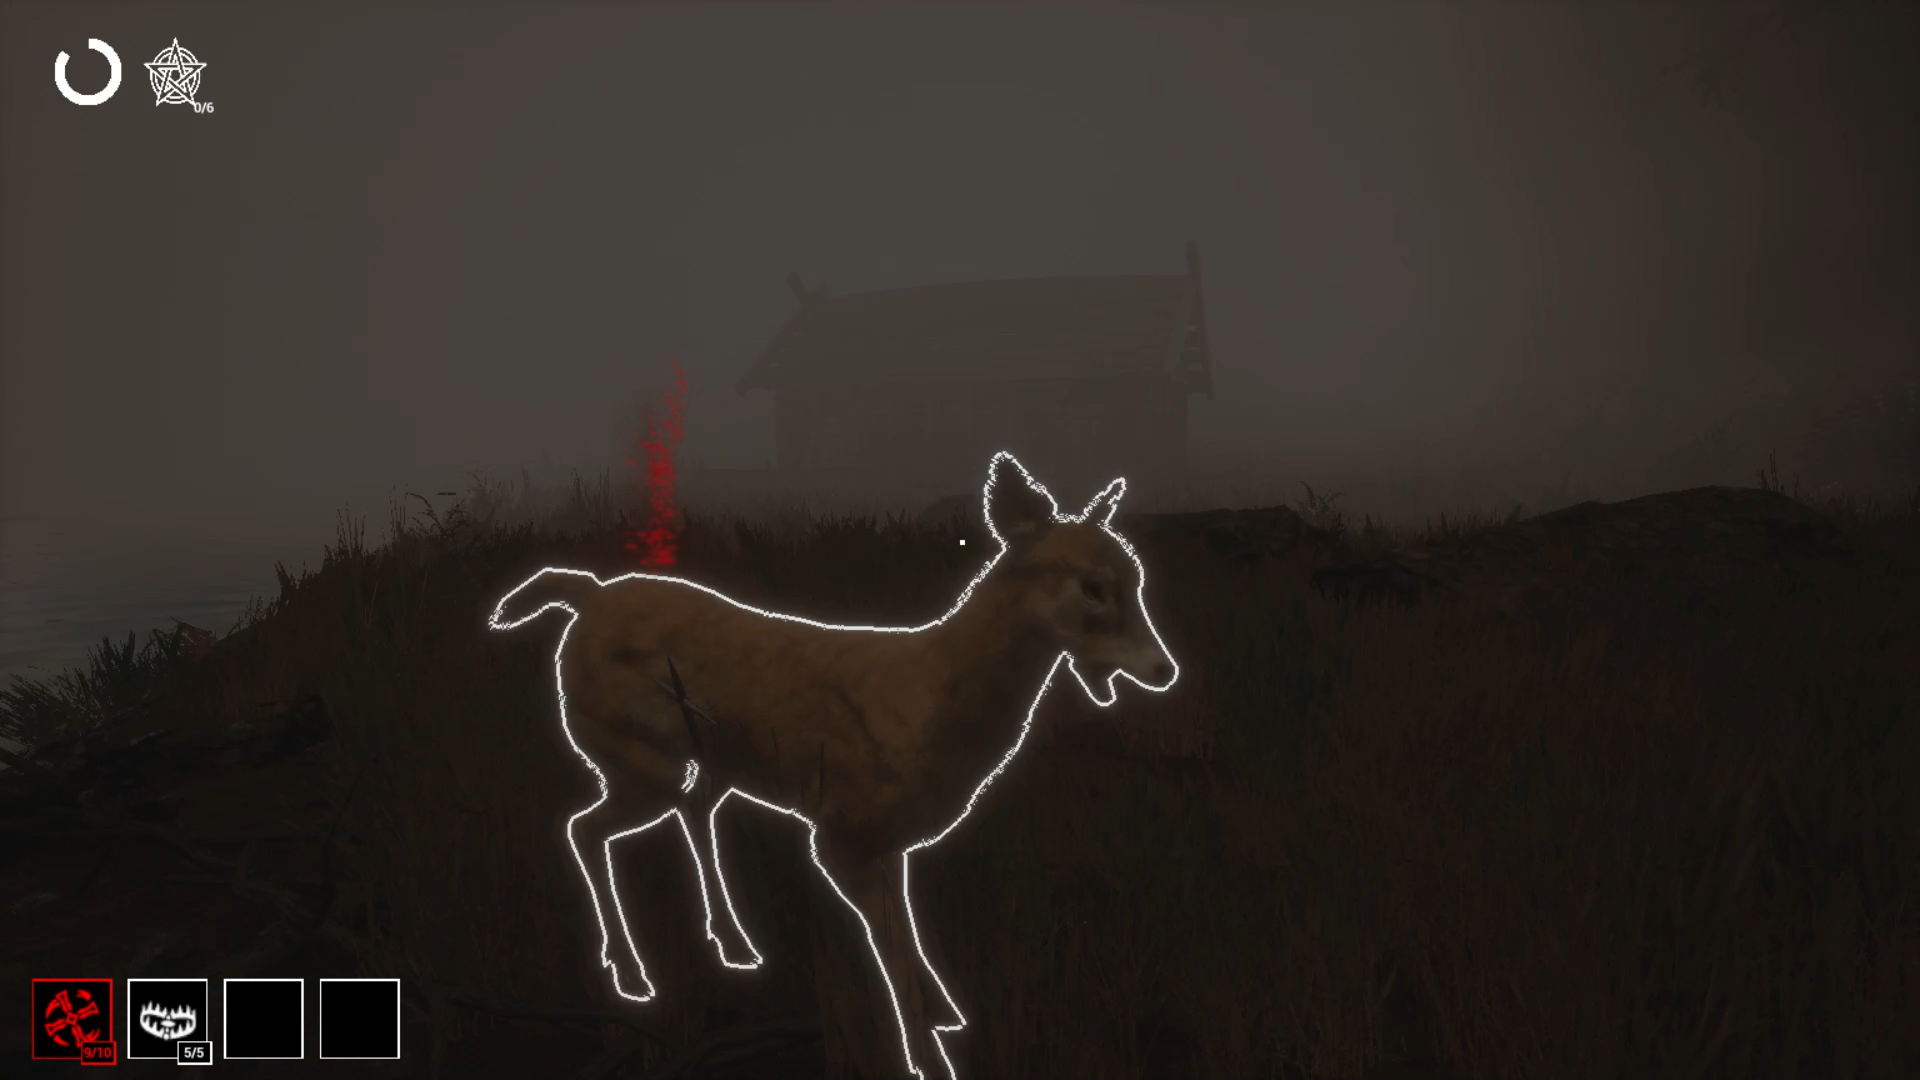
\includegraphics[width=\textwidth]{./img/mechanics/throw_knife_deer.png}
  \end{center}
    \caption[การจับกวางโดยใช้มีด]{การจับกวางโดยใช้มีด}
    \label{fig:การจับกวางโดยใช้มีด}
\end{figure}

\begin{figure}[p]
  \begin{center}
  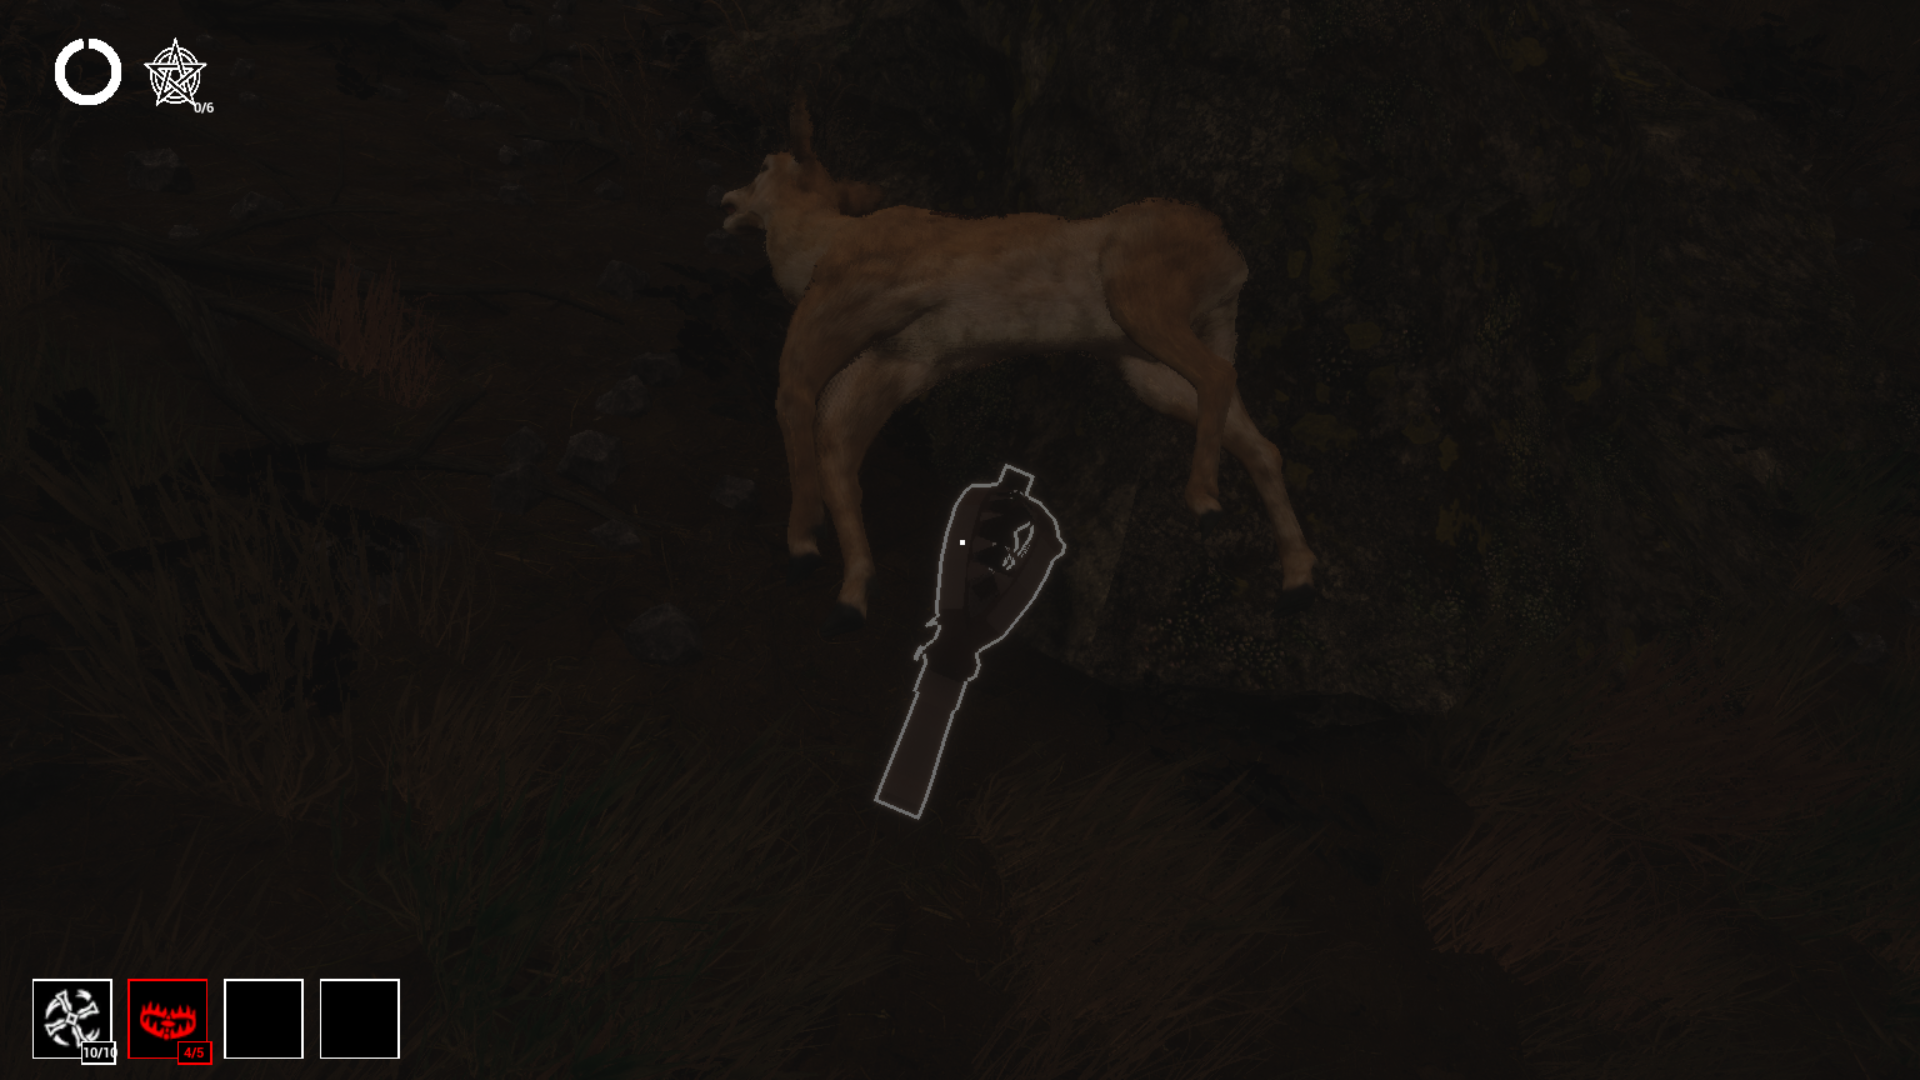
\includegraphics[width=\textwidth]{./img/mechanics/deer_trapped.png}
  \end{center}
    \caption[การจับกวางด้วยกับดัก]{การจับกวางด้วยกับดัก}
    \label{fig:trap}
\end{figure}

\begin{figure}[p]
  \begin{center}
  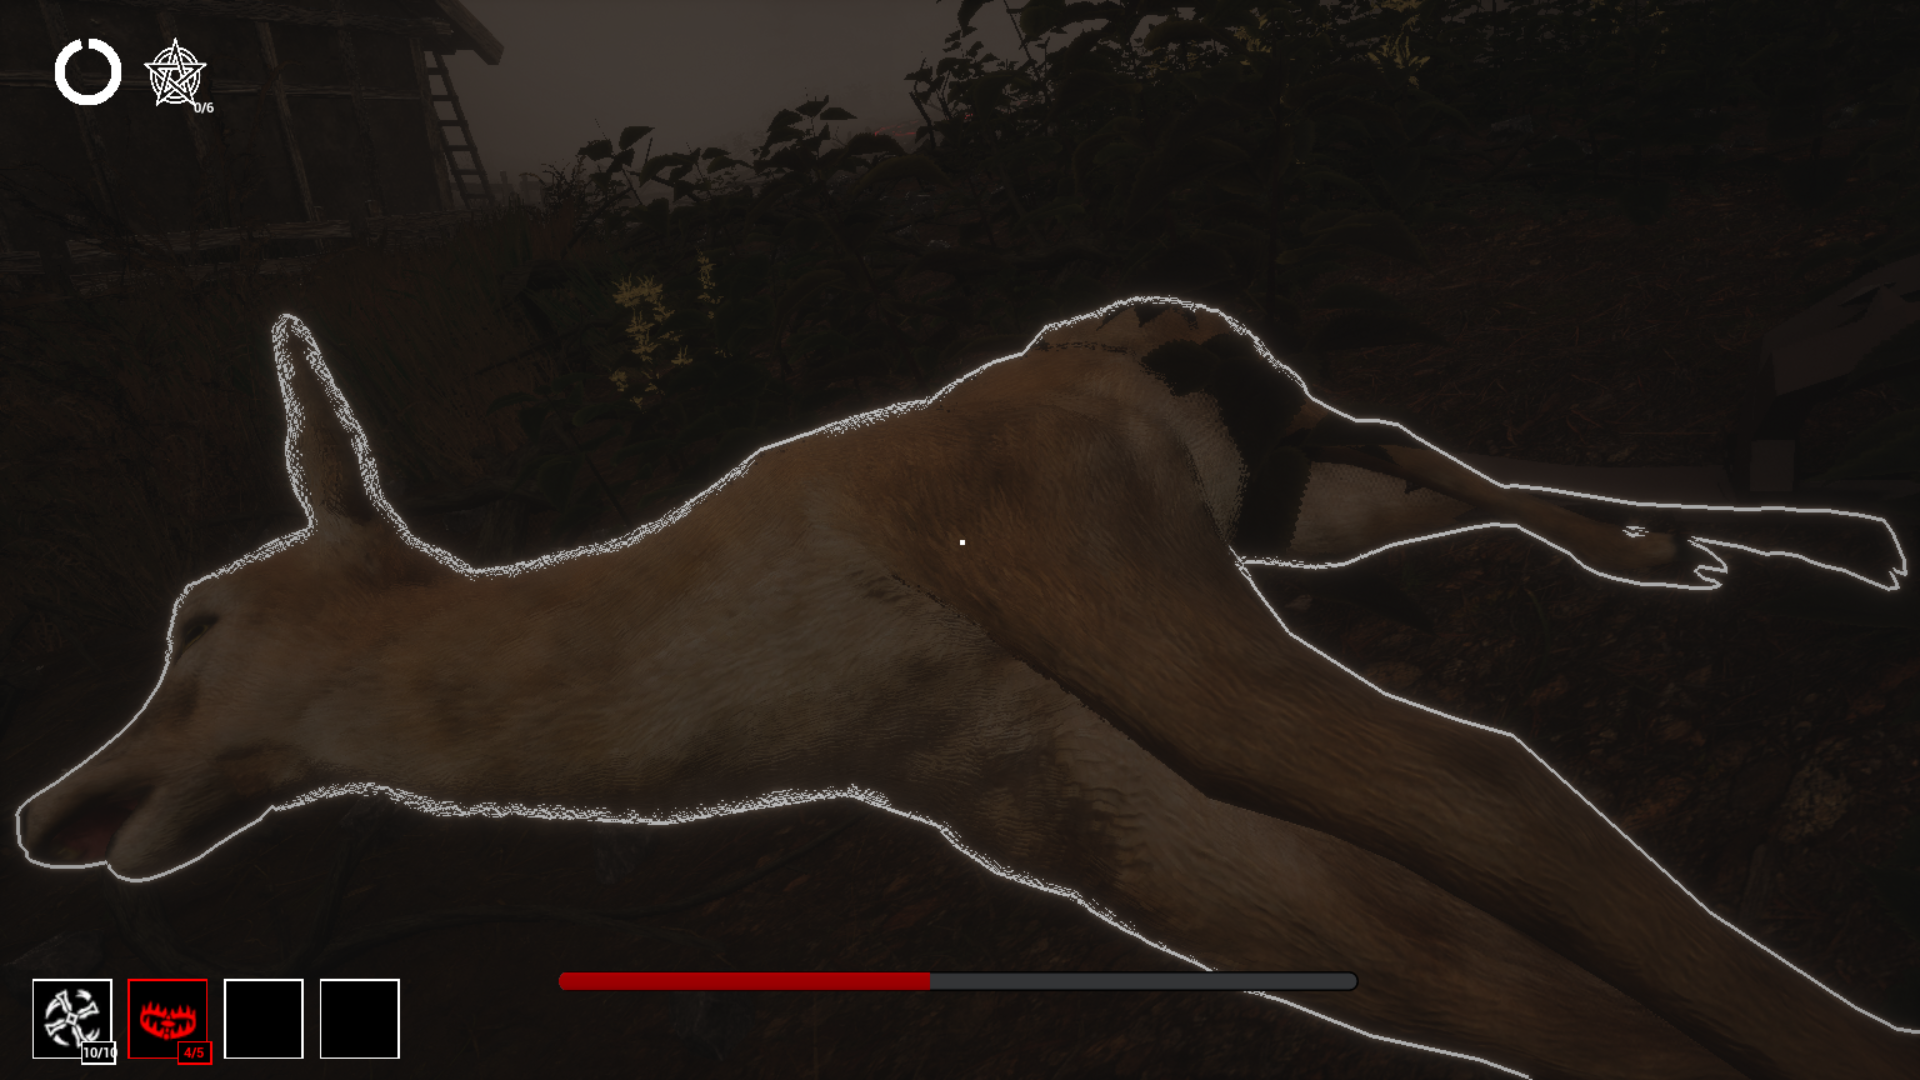
\includegraphics[width=\textwidth]{./img/mechanics/extract_blood.png}
  \end{center}
  \caption[การสกัดเลือดจากตัวกวาง]{การสกัดเลือดจากตัวกวาง}
  \label{fig:blood}
\end{figure}

\subsubsection{การทำพิธี}

เมื่อ Hunter ได้ทำการสกัดเลือดจากกวางแล้ว Hunter สามารถเลือกทำพิธีกรรม โดยการนำเลือดที่สกัดไปทำพิธีตามจุดที่กำหนดไว้จุดไหนก็ได้ ดังแสดงในรูปที่ ~\ref{fig:ritual}
ซึ่งจะมีกำหนดแบบสุ่มไว้ 3 จุด และสามารถทำซ้ำจุดเดิมได้ ซึ่งเมื่อผู้เล่นคนนั้นทำพิธีเสร็จสิ้นแล้ว 1 ครั้ง เขาจะได้รับการฟื้นฟู 
HP 1 ระดับ ในการทำพิธี 1 ครั้งจะใช้เวลา 30 วินาที สามารถยกเลิกการทำพิธีได้ แต่ต้องเริ่มทำพิธีใหม่ทั้งหมด

\begin{figure}[h]
  \begin{center}
  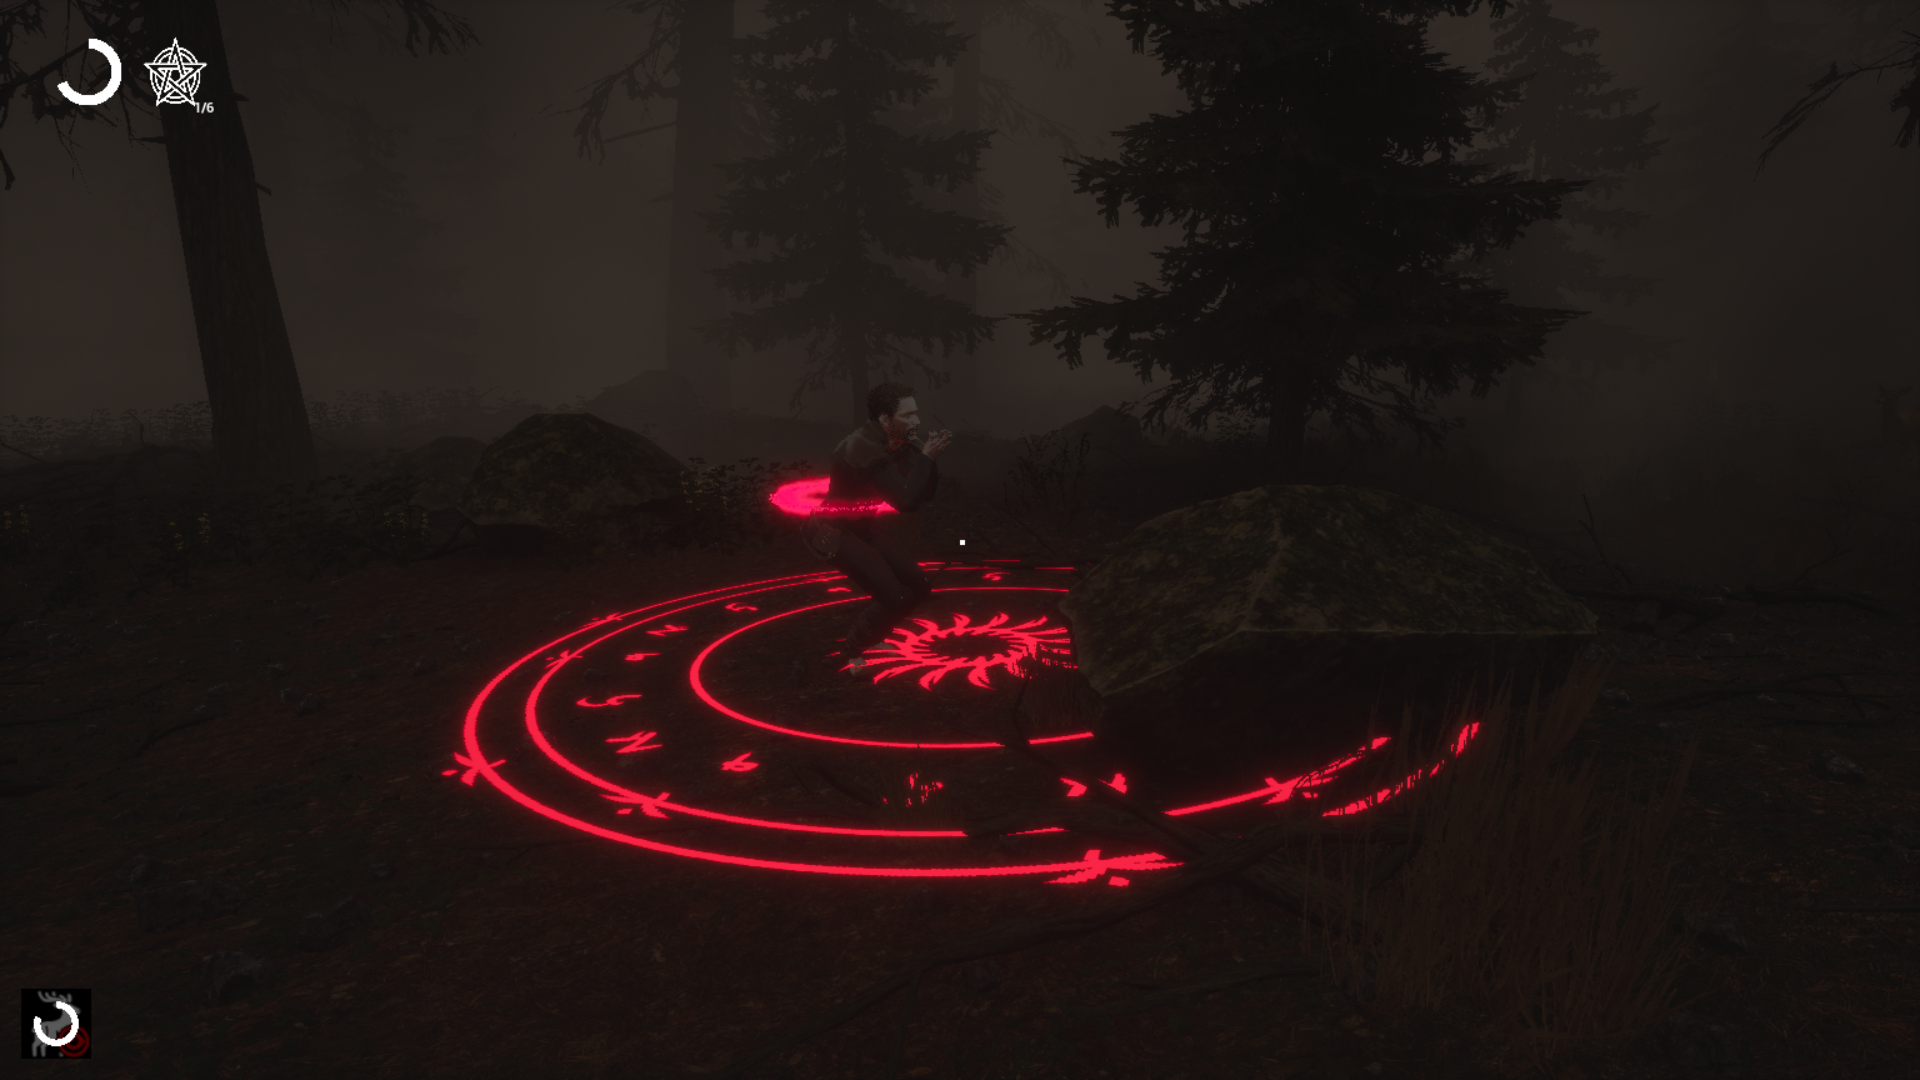
\includegraphics[width=\textwidth]{./img/mechanics/ritual-complete.png}
  \end{center}
  \caption[ภาพการทำพิธีของ Hunter จากมุมมองของผู้เล่นอีกคน]{ภาพการทำพิธีของ Hunter จากมุมมองของผู้เล่นอีกคน}
  \label{fig:ritual}
\end{figure}

\subsubsection{การโจมตี Witch}

Hunter สามารถโจมตี Witch ได้ด้วยการปามีดศักดิ์สิทธิ์ใส่ Witch หรือปักไว้ที่พื้นเพื่อล่อให้ Witch มาเหยียบ การโจมตี Witch นี้จะทำให้ Witch สะดุดและเดินช้าลง 
รวมถึงทำให้มองไม่เห็นชั่วครู่ ดังแสดงในรูปที่ \ref{fig:blind} ในระหว่างนี้ Hunter สามารถวิ่งไปแอบหลังต้นไม้หรือก้อนหิน เพื่อหลุดจากการไล่ล่าและทำพิธีต่อ

\begin{figure}[h]
  \begin{center}
  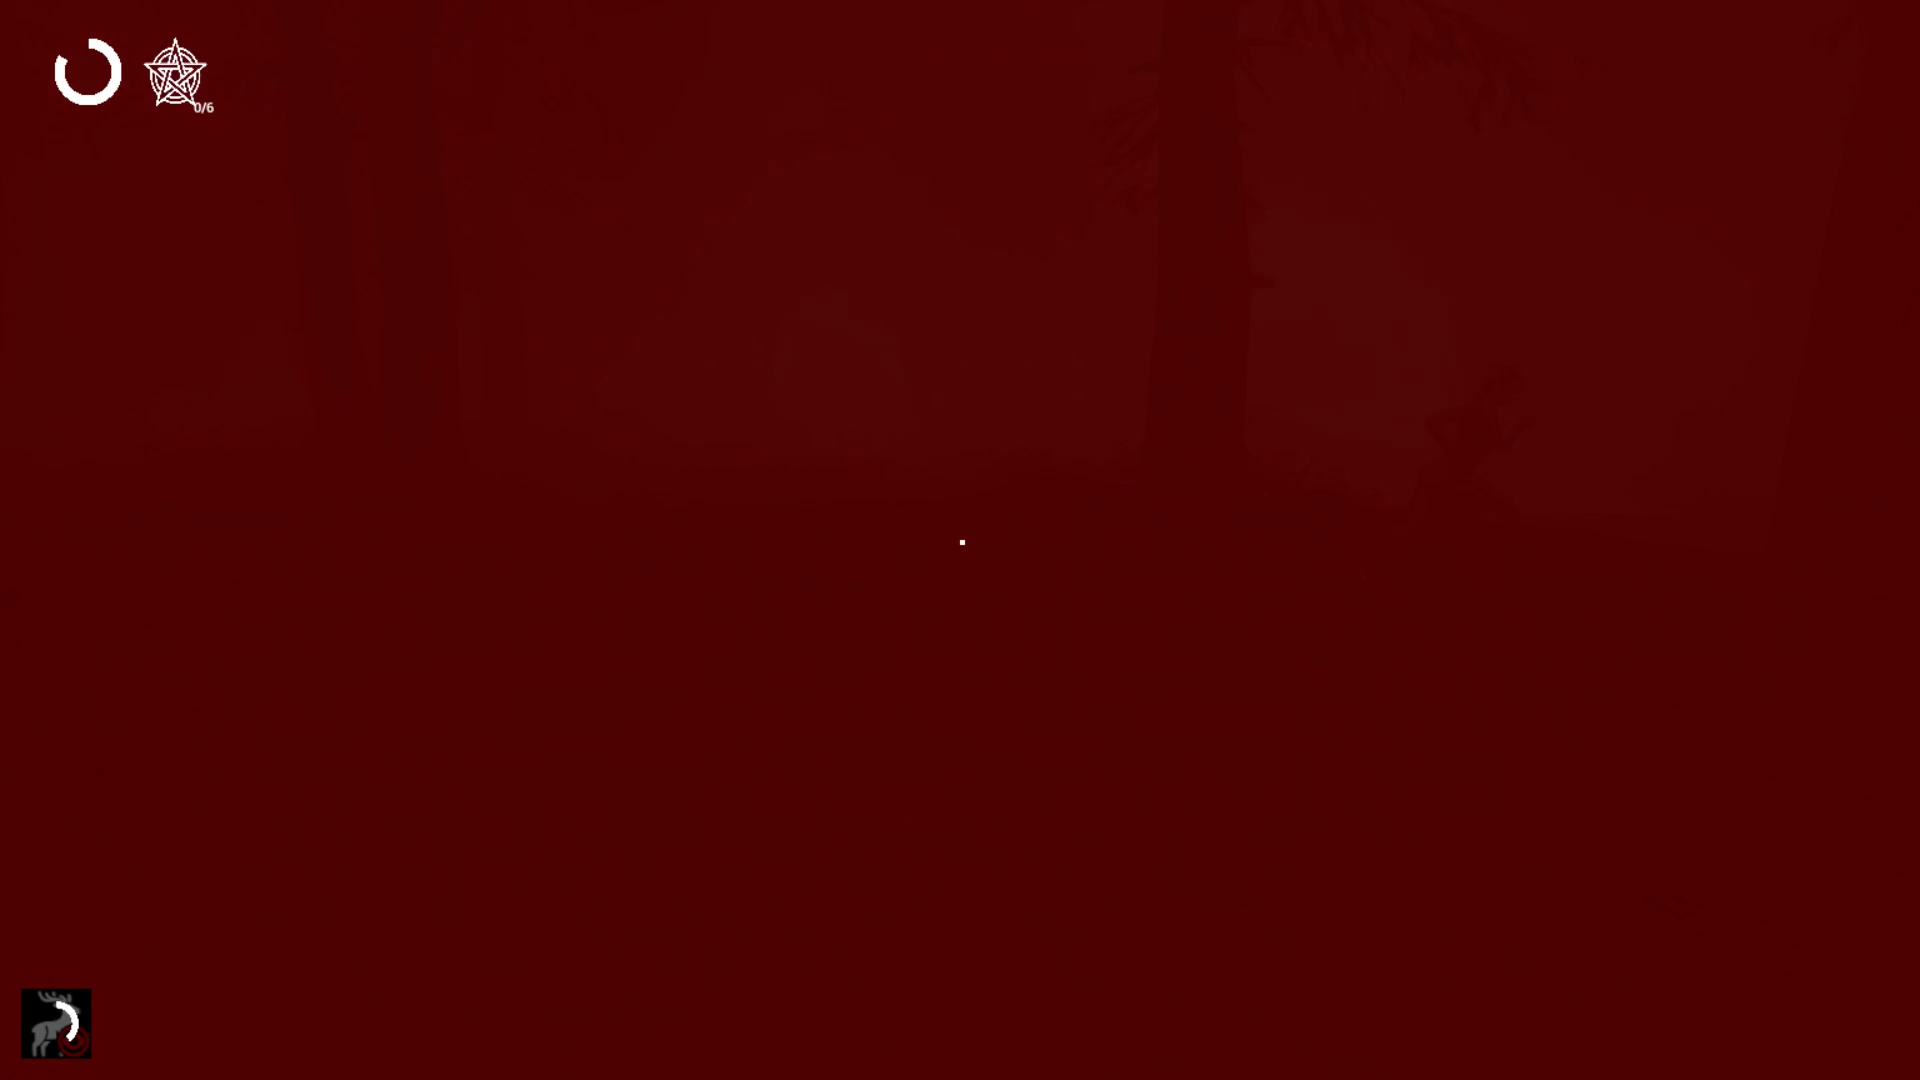
\includegraphics[width=\textwidth]{./img/mechanics/witch_blind.png}
  \end{center}
  \caption[Witch จะตาบอดและเดินไม่ได้ชั่วครู่เมื่อถูกโจมตี]{Witch จะตาบอดและเดินไม่ได้ชั่วครู่เมื่อถูกโจมตี}
  \label{fig:blind}
\end{figure}

\subsubsection{ระบบ Inventory}

Hunter สามารถเก็บ ใช้ และดร็อปไอเทมได้ ทำให้สามารถส่งต่อไอเทมให้ผู้เล่นอีกคนได้อีกด้วย Inventory มีทั้งหมด 4 ช่องตามรูปที่ ~\ref{fig:inventory} และไม่สามารถขยายได้เมื่อช่องเต็มแล้ว
โดยไอเทมที่สามารถเก็บและใช้ได้ มีดังนี้
\begin{enumerate}
  \item มีดศักดิ์สิทธิ์ มีให้ 10 เล่ม stack ได้ 10 เล่ม ปามีดแล้วสามารถเก็บมาใช้ซ้ำได้
  \item กับดักสัตว์ มีให้ 5 อัน stack ได้ 5 อัน กับดับสามารถวางไว้ได้ทุกที่ และสามารถเก็บมาใช้ซ้ำได้
  \item หลอดบรรจุเลือดของกวางที่ได้หลังจากการสกัดเลือด stack ได้ 3 หลอด
\end{enumerate}

\begin{figure}[h]
  \begin{center}
  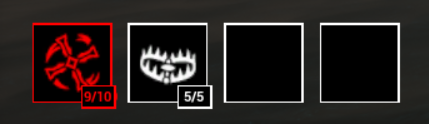
\includegraphics[width=0.5\textwidth]{./img/mechanics/inventory.png}
  \end{center}
  \caption[ระบบ Inventory]{ระบบ Inventory}
  \label{fig:inventory}
\end{figure}

\subsubsection{ระบบ HP}

HP ของ Hunter มี 3 ระดับ โดยเมื่อถูกโจมตีจาก Witch จะลดลง 1 ระดับ และสามารถฟื้นฟู HP 1 ระดับได้ด้วยการทำพิธี 
1 ครั้ง แต่ไม่สามารถฟื้นฟู HP จนมากกว่า 3 ระดับได้

ในเกมจะไม่แสดงหลอดเลือดแต่แสดงเป็น Vignette Effect สีแดงบนจอตามรูปที่ ~\ref{fig:damage_effect} ซึ่งจะรุนแแรงขึ้นเรื่อย ๆ ตามระดับ HP ที่ลดลงไป

\begin{figure}[p]
  \begin{center}
  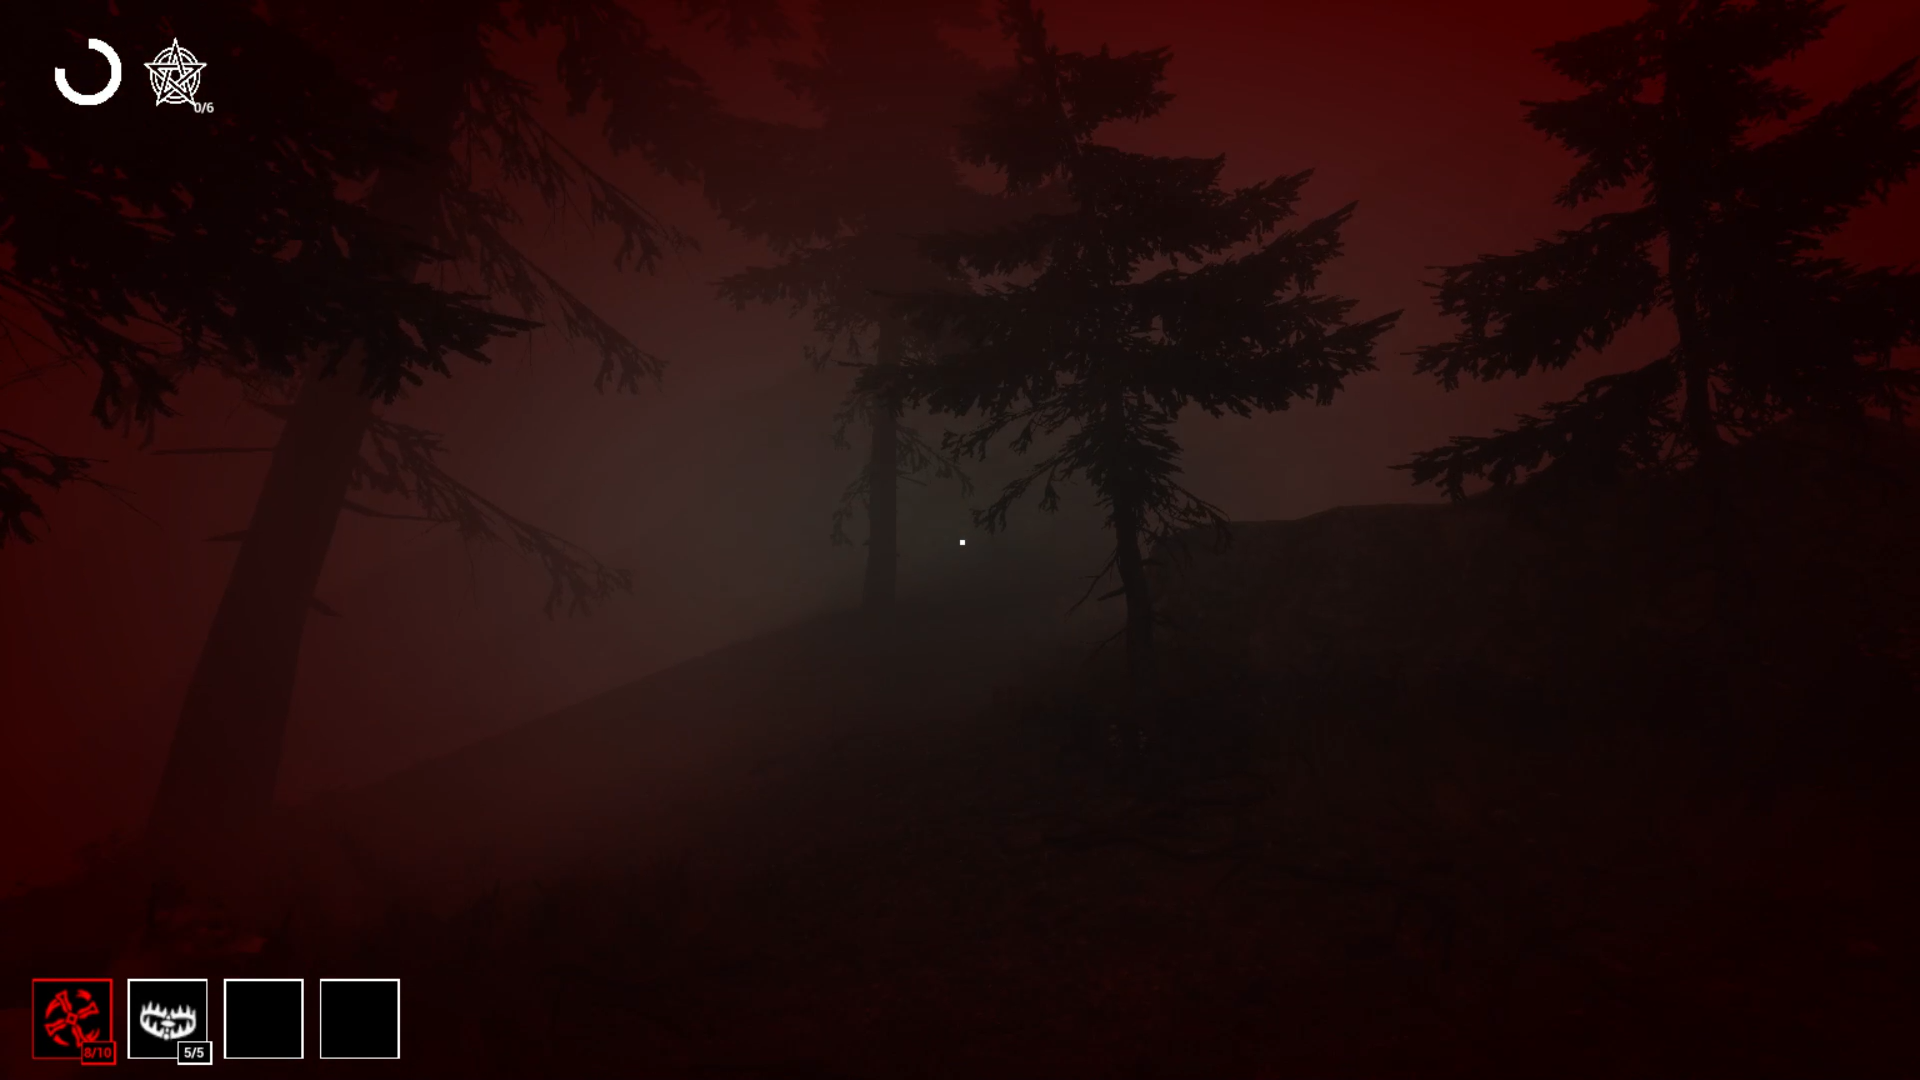
\includegraphics[width=\textwidth]{./img/mechanics/damage_effect.png}
  \end{center}
  \caption[Effect เมื่อ Hunter บาดเจ็บ]{Effect เมื่อ Hunter บาดเจ็บ}
  \label{fig:damage_effect}
\end{figure}

\subsubsection{ระบบชุบชีวิต}

เมื่อ Hunter ไม่เหลือ HP แล้ว จะเข้าสู่สถานะชุบชีวิต Hunter จะเกิดใหม่เป็นร่างวิญญาณ ณ ร่างของผู้เล่นอีกคน 
สามารถเลือกที่จะเกิดใหม่ด้วยการเดินกลับไปสิงร่างเดิม หรือเลือกที่จะไม่เกิดใหม่แต่เล่นเป็น Spectator ได้ ผู้เล่นคนอื่น ๆ 
จะไม่สามารถเห็น Hunter ในร่างวิญญาณนี้ Hunter แต่ละคนสามารถชุบชีวิตได้เพียง 1 ครั้งเท่านั้น มุมมองของผู้เล่นที่เป็นร่างวิญญาณ แสดงในรูปที่ ~\ref{fig:revive}

\begin{figure}[p]
  \begin{center}
  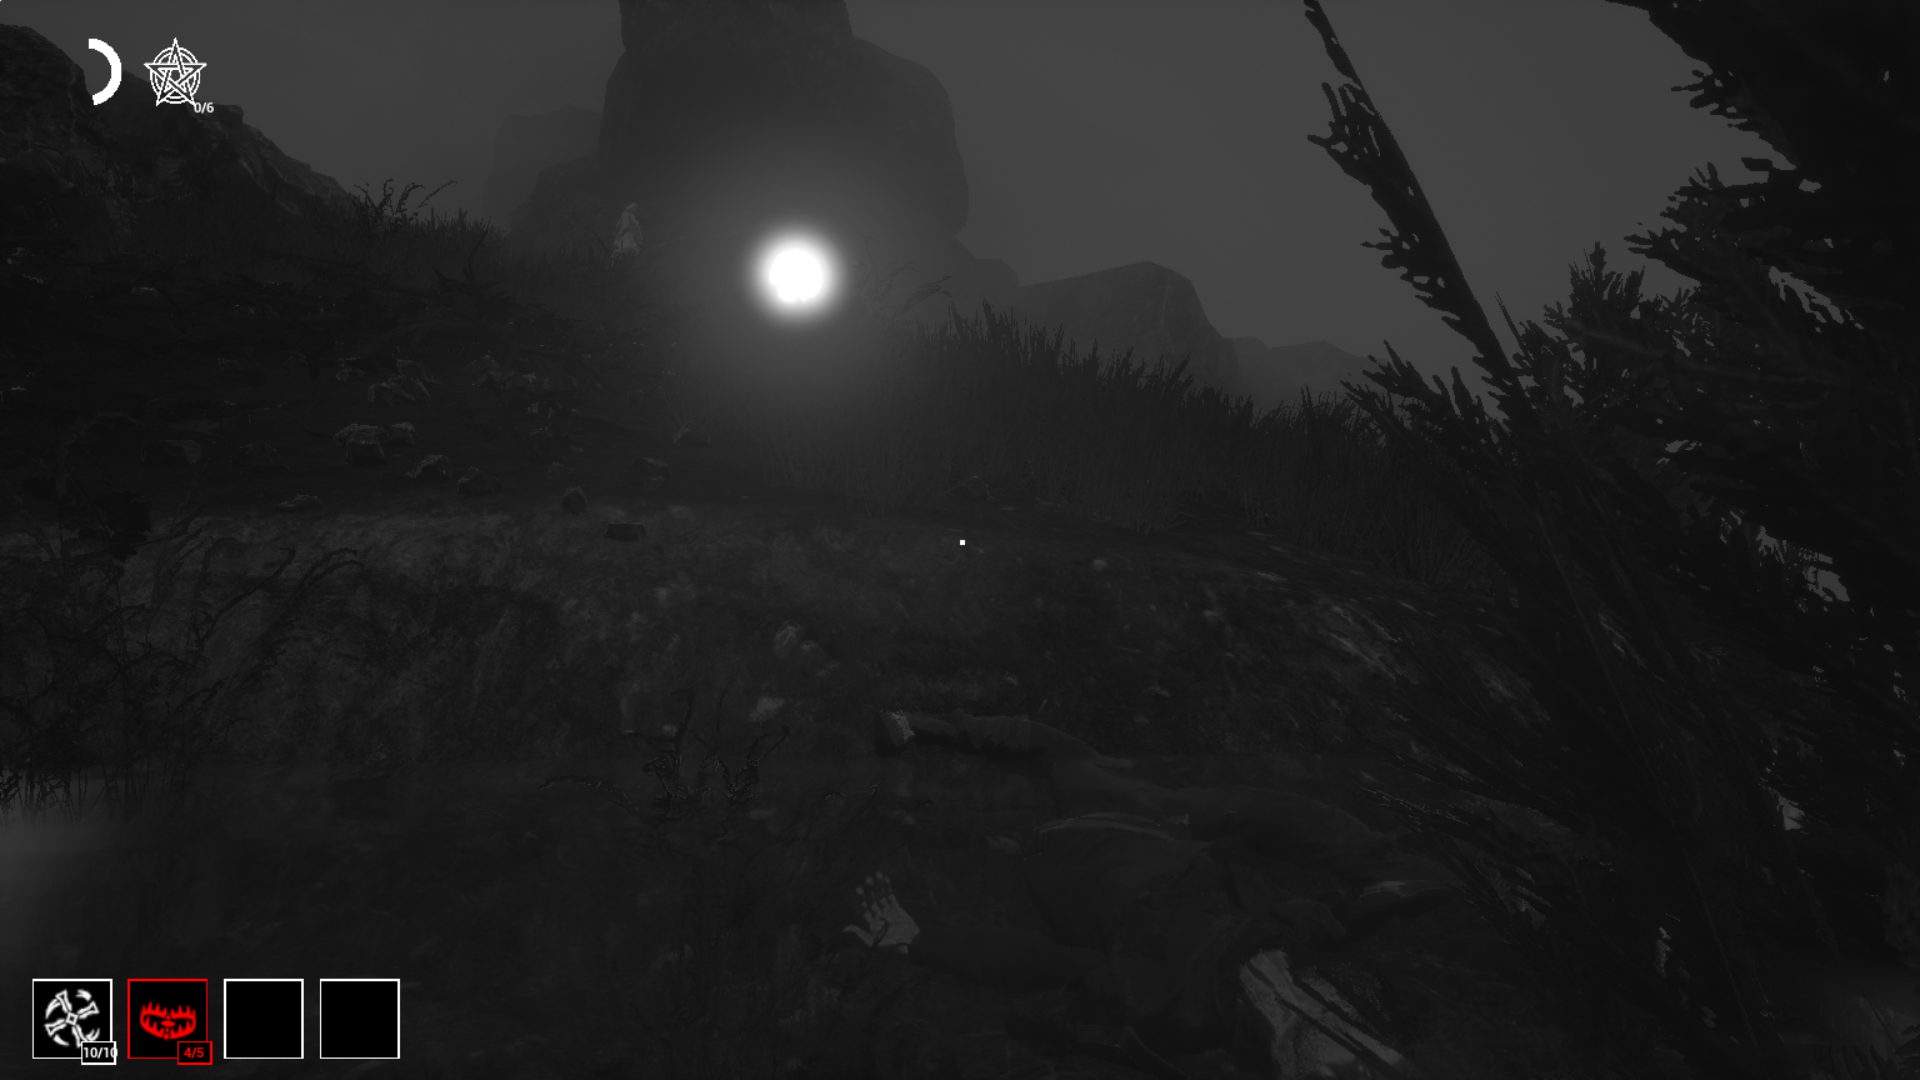
\includegraphics[width=\textwidth]{./img/mechanics/revive.png}
  \end{center}
  \caption[ภาพแสดงมุมมองของผู้เล่นที่เป็นร่างวิญญาณ ต้องสิงกลับร่างเดิมเพื่อชุบชีวิต]{ภาพแสดงมุมมองของผู้เล่นที่เป็นร่างวิญญาณ ต้องสิงกลับร่างเดิมเพื่อชุบชีวิต}
  \label{fig:revive}
\end{figure}

\subsection{การเล่นของฝ่าย Witch}

\subsubsection{การโจมตี Hunter}

Witch สามารถโจมตี Hunter ได้โดยการใช้เวทมนต์ 2 แบบ แบบระยะใกล้และระยะไกล โดยเมื่อโจมตีแล้ว 
Hunter จะลด HP ลง 1 ระดับ

\begin{enumerate}
  \item การโจมตีระยะใกล้ด้วยไอพิษ (Breath of Death): สามารถโจมตีได้ในระยะ 1-2 เมตร การโจมตีเป็นรูปแบบของการพ่นไอพิษ ดังแสดงในรูปที่ ~\ref{fig:short_range_attack}
  \item การโจมตีระยะไกลด้วยลูกไฟ (Inferno Soul): สามารถโจมตีในระยะไกลเท่าไหร่ก็ได้ การโจมตีเป็นรูปแบบของการยิงเวทมนต์ไฟ ดังแสดงในรูปที่ ~\ref{fig:long_range_attack}
(Fire Ball) โดยจะต้องมีการชาร์จพลังให้เต็มก่อนที่จะโจมตีในทุกครั้ง
\end{enumerate}

\begin{figure}[p]
  \begin{center}
  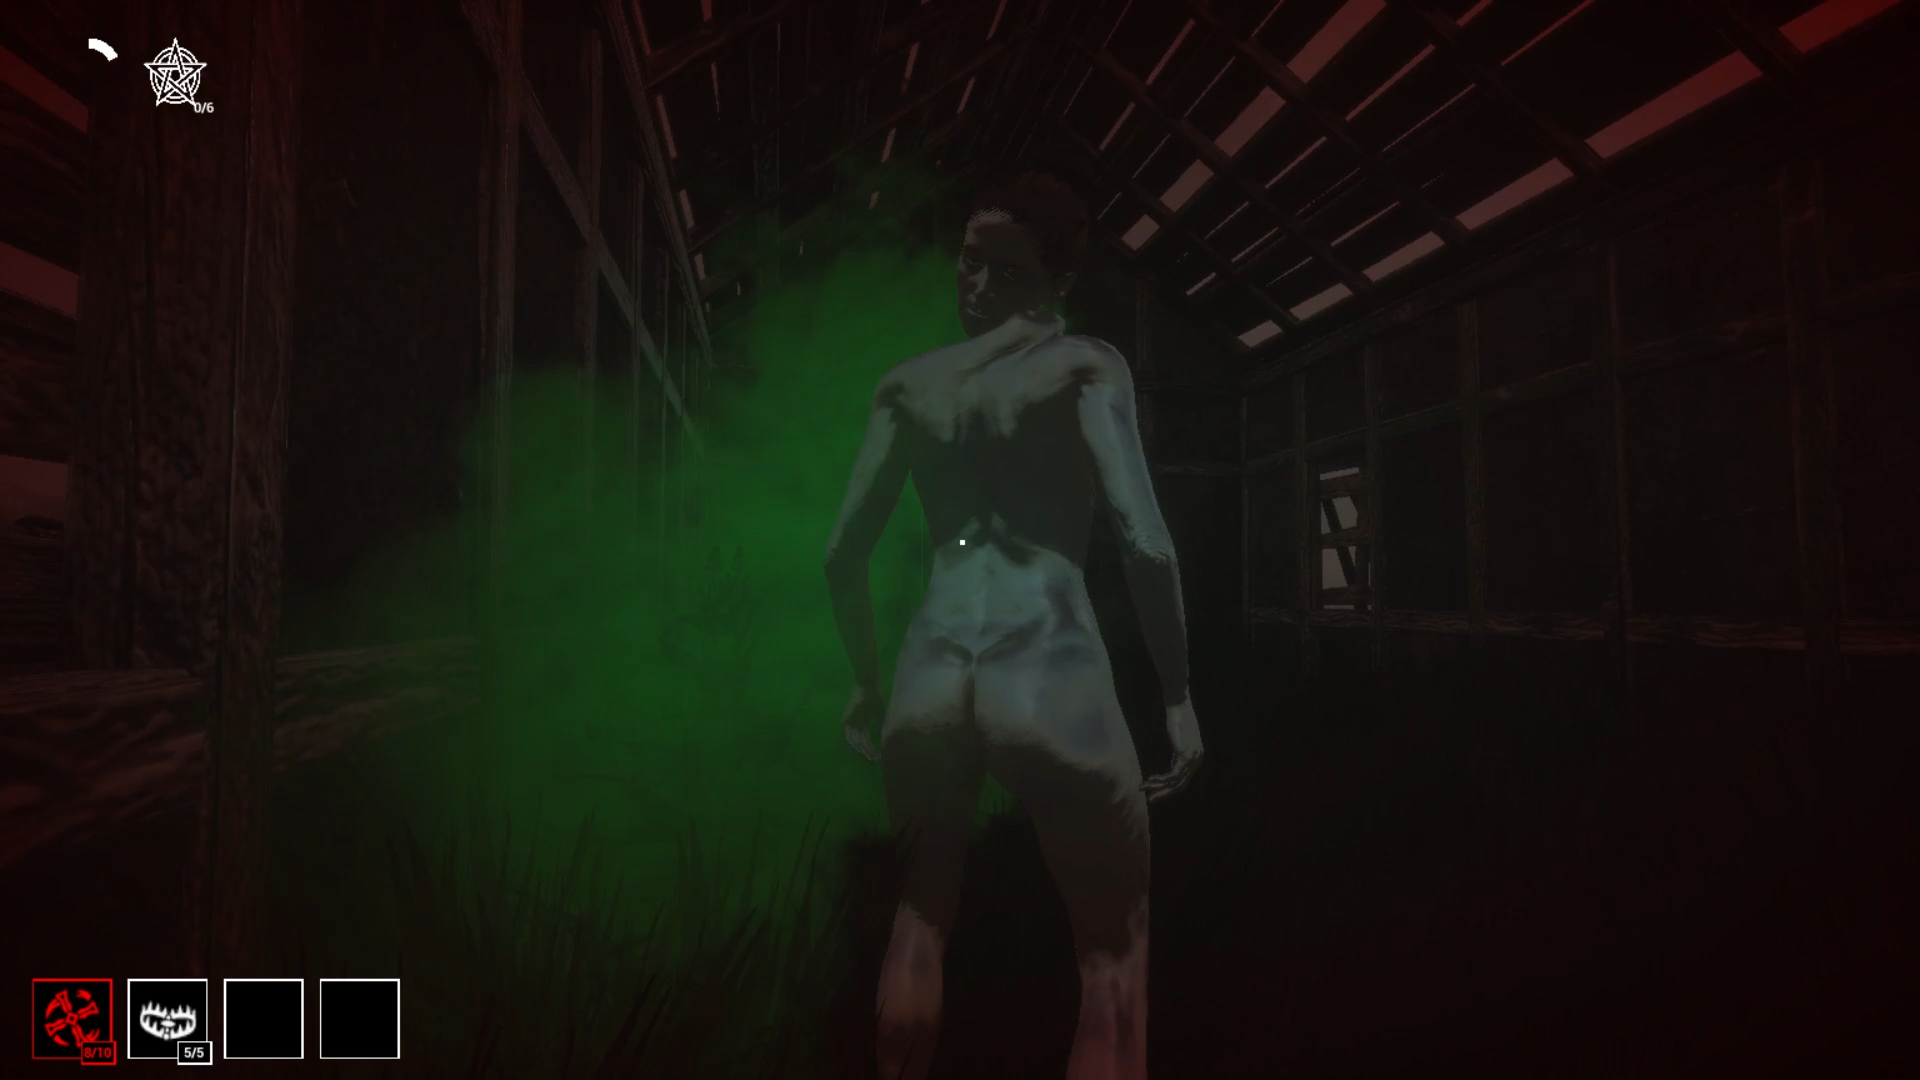
\includegraphics[width=\textwidth]{./img/mechanics/breath_of_death.png}
  \end{center}
    \caption[การโจมตีระยะใกล้ด้วยไอพิษของ Witch]{การโจมตีระยะใกล้ด้วยไอพิษของ Witch}
    \label{fig:short_range_attack}    
\end{figure}

\begin{figure}[p]
  \begin{center}
  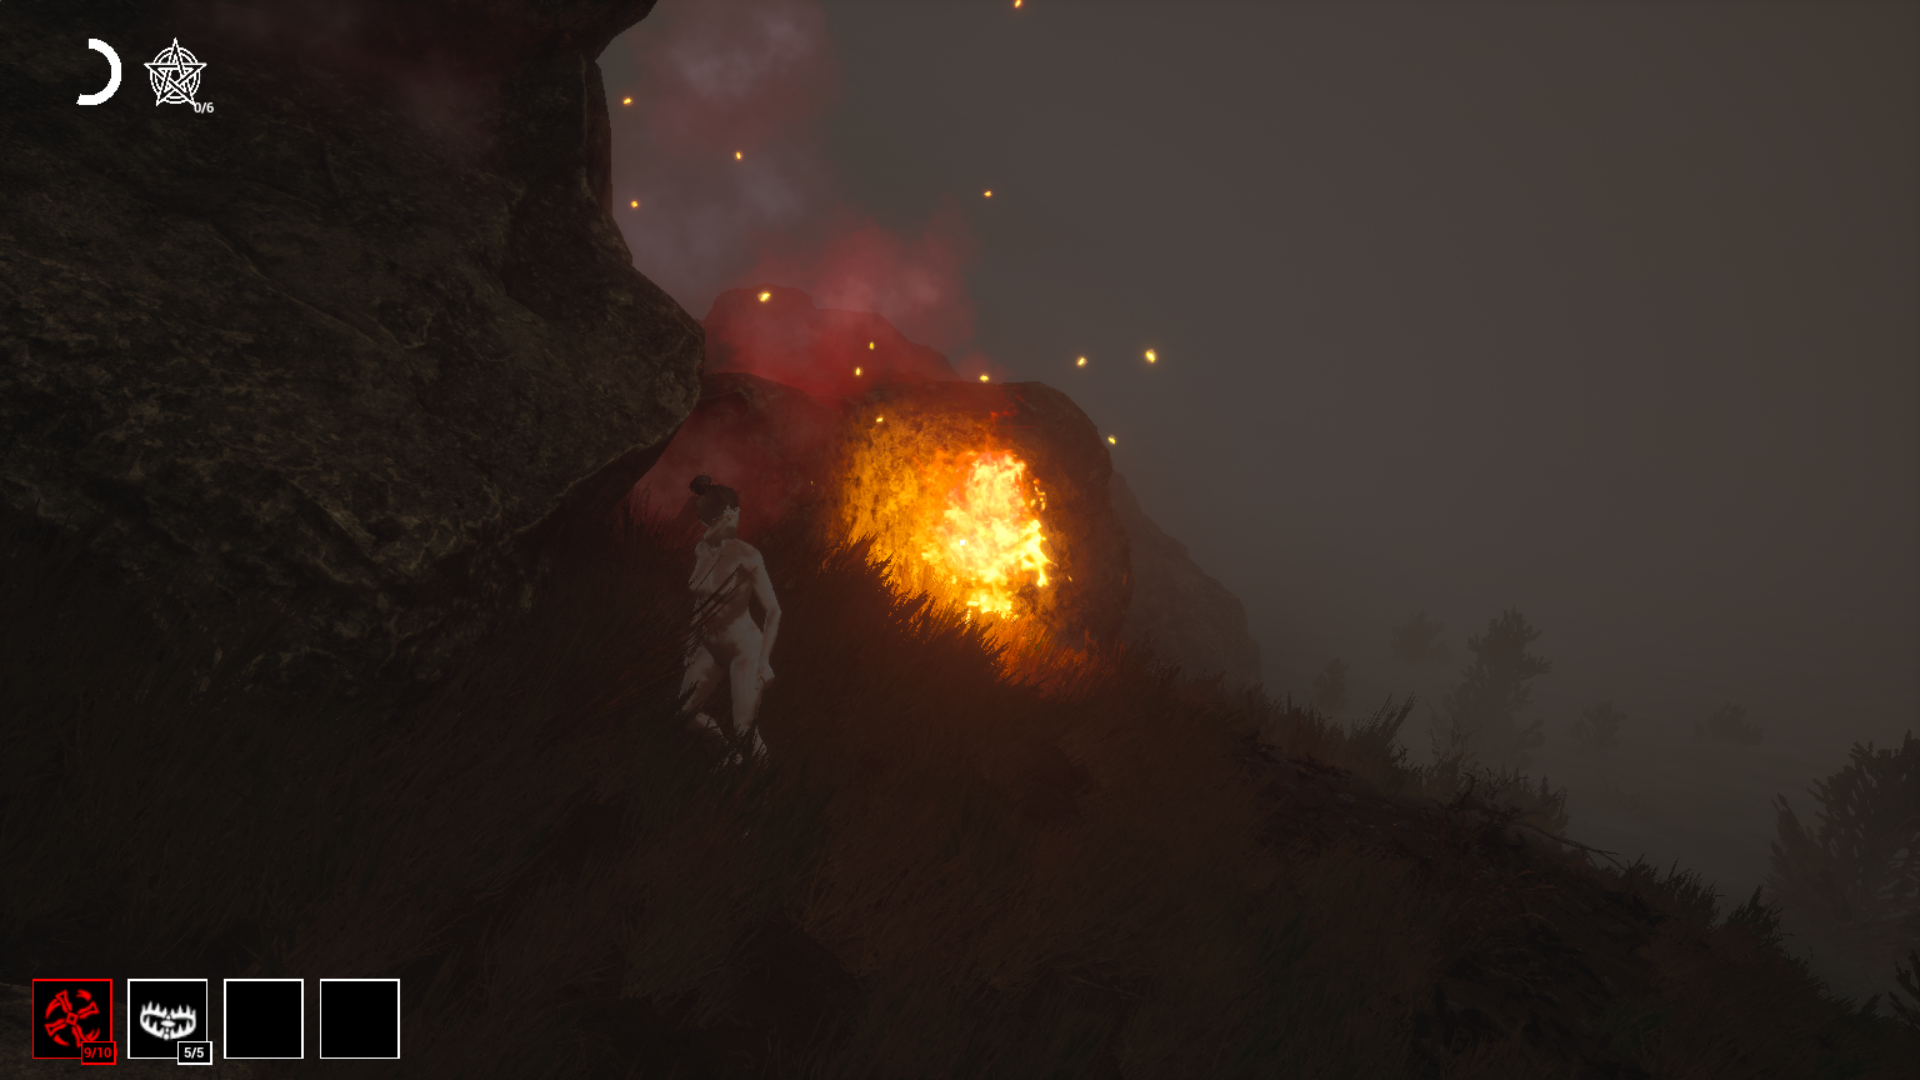
\includegraphics[width=\textwidth]{./img/mechanics/inferno_soul.png}
  \end{center}
    \caption[การโจมตีระยะไกลด้วยลูกไฟของ Witch]{การโจมตีระยะไกลด้วยลูกไฟของ Witch}\label{การโจมตีระยะไกลด้วยลูกไฟ}
    \label{fig:long_range_attack}
\end{figure}

\subsubsection{การเคลื่อนย้ายร่างไปเป็นกวาง}

Witch สามารถกดดูตำแหน่งและการเคลื่อนที่ของกวางในแมพได้ (Deer Vision) ดังแสดงในรูปที่ ~\ref{fig:deer_vision} ซึ่งสามารถใช้เลือกกวางที่จะย้ายร่างไปสิงได้
ความสามารถนี้สามารถใช้ได้ทุก ๆ 60 วินาที ในขณะเป็นกวางอยู่ ผู้เล่นไม่สามารถทำการโจมตีอีกฝั่งได้
ต้องกลับมาเป็นร่าง Witch เดิมก่อนทำการโจมตี ถ้าหากกวางที่ผู้เล่นสิงอยู่ถูกโจมตีจะทำให้วิญญาณกลับมาเป็นร่างเดิมทันที

\begin{figure}[p]
  \begin{center}
  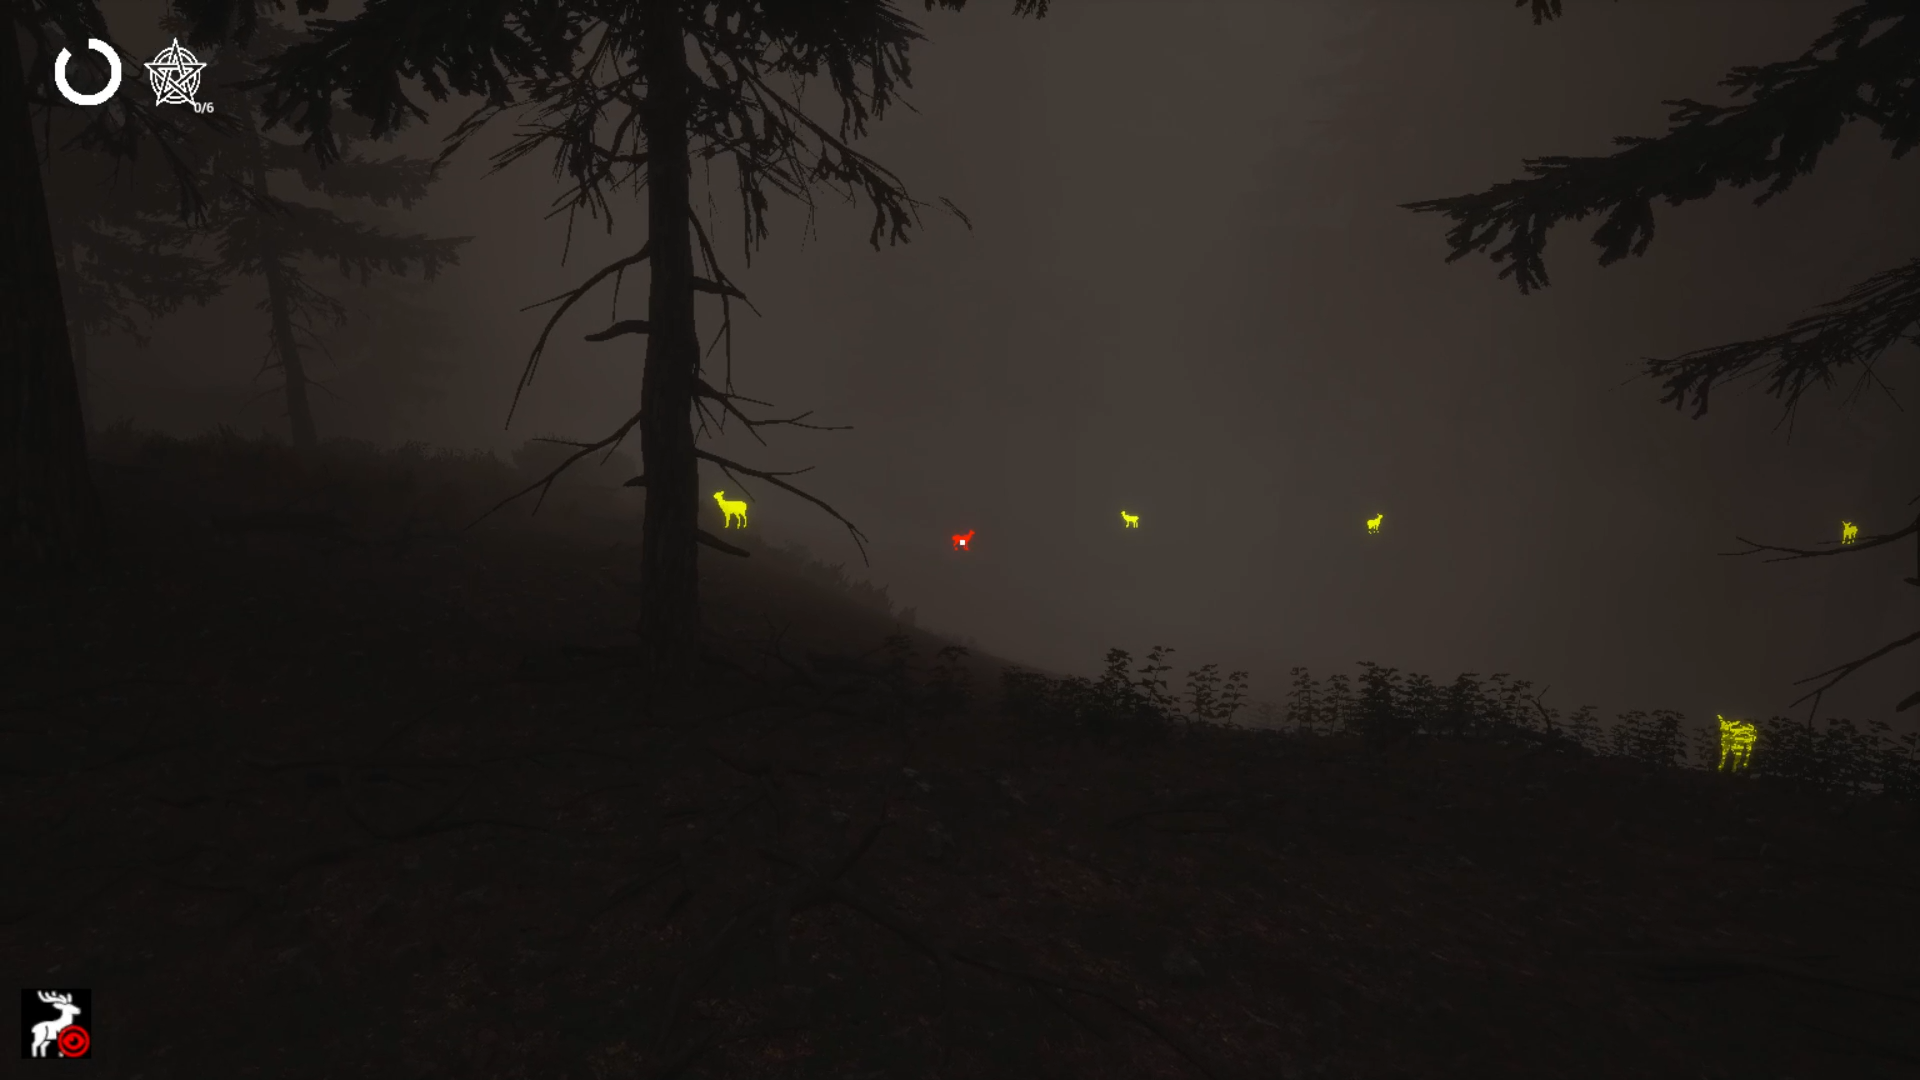
\includegraphics[width=\textwidth]{./img/mechanics/deervision.png}
  \end{center}
    \caption[Witch ใช้ความสามารถดูตำแหน่งของกวางที่สามารถสิงร่างได้ (Deer Vision)]{Witch ใช้ความสามารถดูตำแหน่งของกวางที่สามารถสิงร่างได้ (Deer Vision)}
    \label{fig:deer_vision}
\end{figure}

\begin{figure}[p]
  \begin{center}
  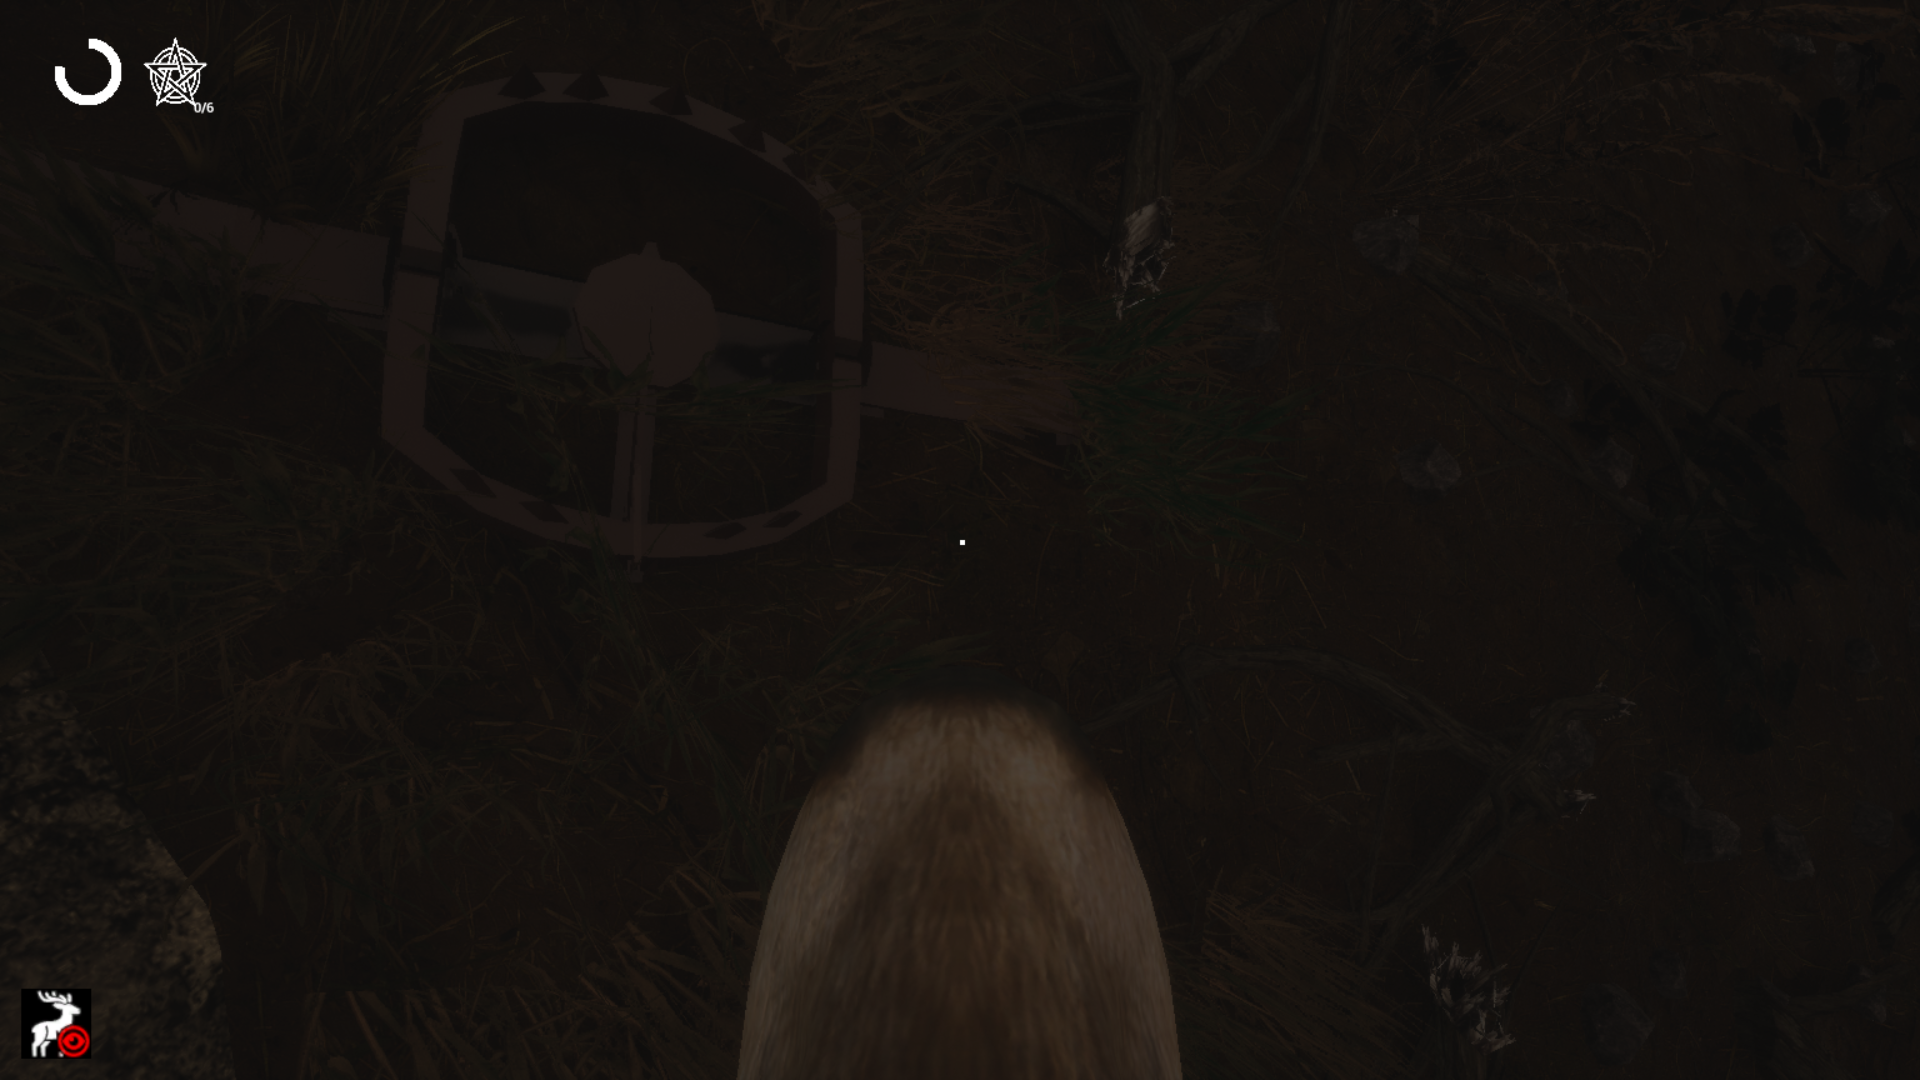
\includegraphics[width=\textwidth]{./img/mechanics/witch_deer.png}
  \end{center}
    \caption[มุมมองบุคคลที่หนึ่งของ Witch ที่เล่นเป็นกวาง]{มุมมองบุคคลที่หนึ่งของ Witch ที่เล่นเป็นกวาง}
    \label{fig:deer_view}
\end{figure}

\subsubsection{ความสามารถพิเศษอื่น ๆ}

\begin{itemize}
  \item สามารถมองเห็นตำแหน่งของจุดทำพิธีตอนเริ่มเกมได้ ดังแสดงในรูปที่ ~\ref{fig:see_ritual}
  \item สามารถได้ยินเสียงจุดทำพิธีและการทำพิธีได้ในระยะที่ค่อนข้างไกล
\end{itemize}

\begin{figure}[h]
  \begin{center}
  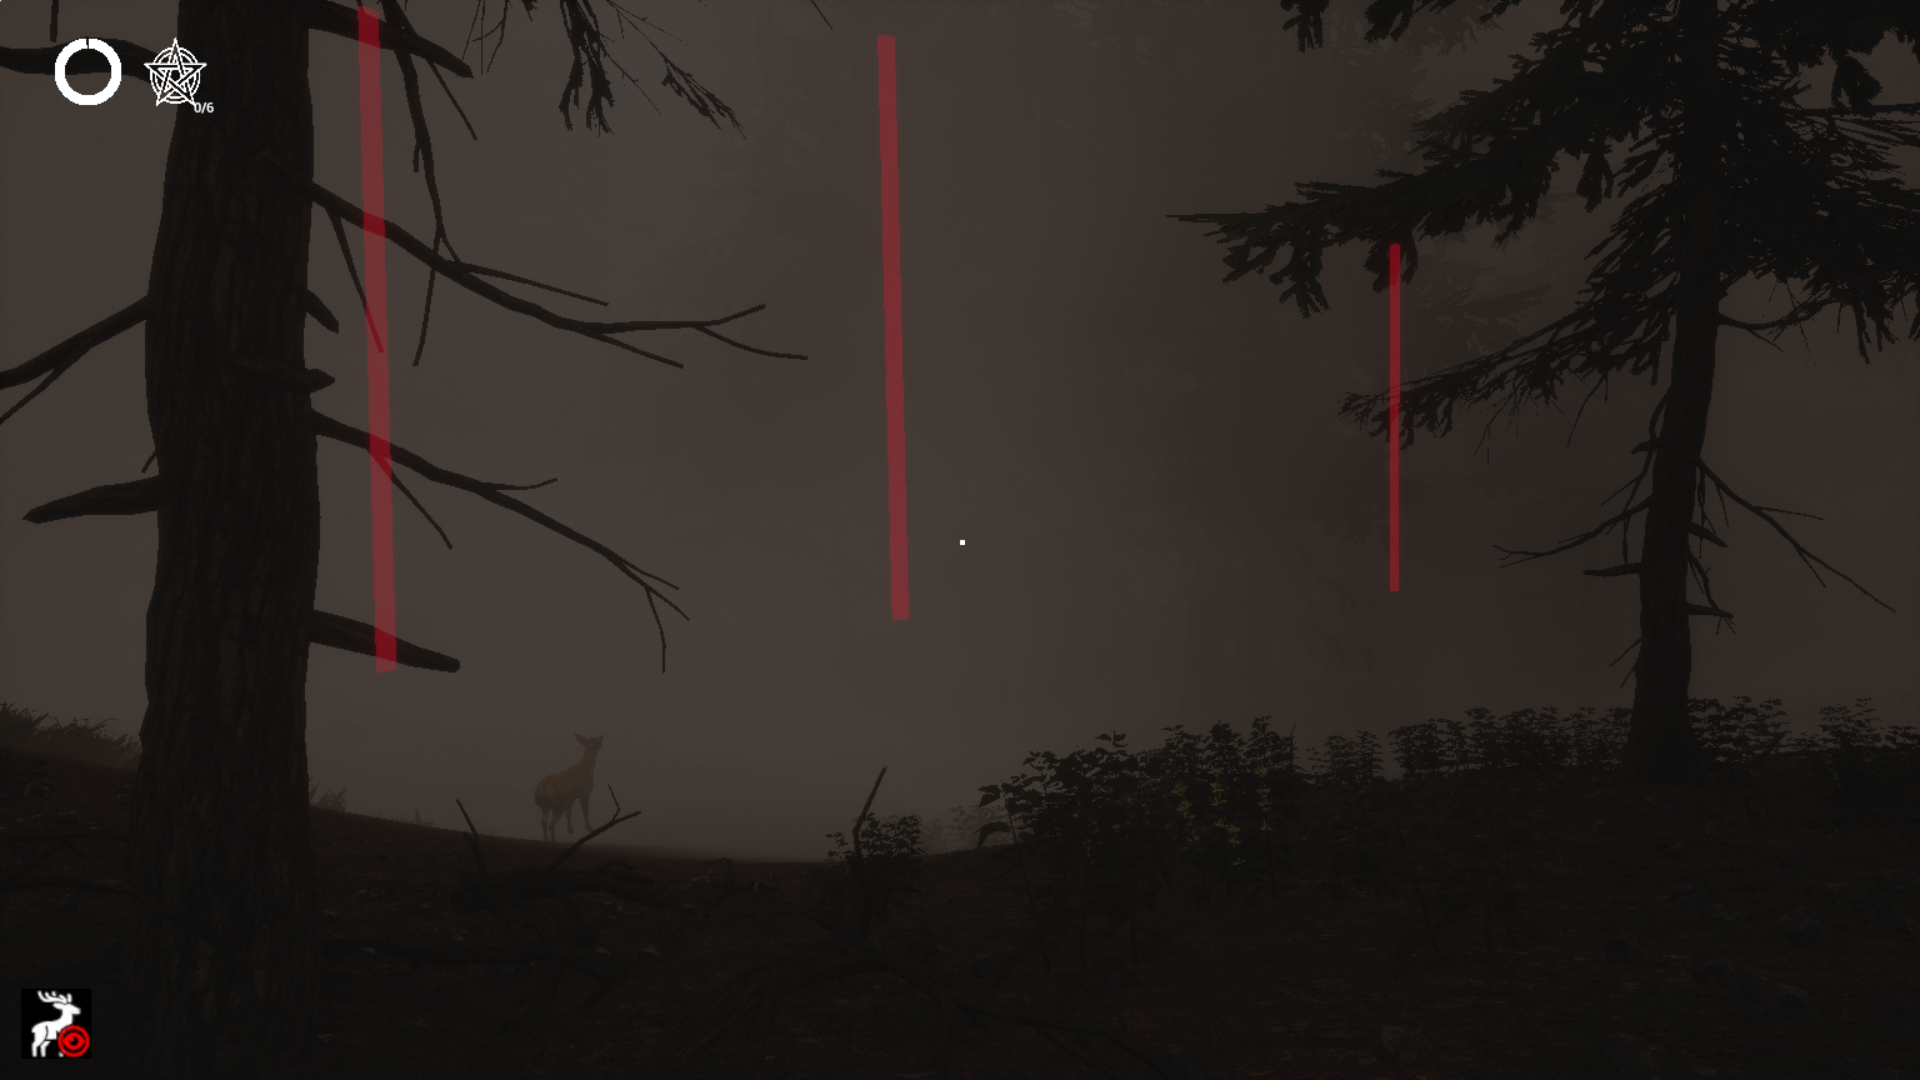
\includegraphics[width=\textwidth]{./img/mechanics/see_ritual.png}
  \end{center}
  \caption[Witch สามารถมองเห็นตำแหน่งของจุดทำพิธีตอนเริ่มเกมได้]{Witch สามารถมองเห็นตำแหน่งของจุดทำพิธีตอนเริ่มเกมได้}
  \label{fig:see_ritual}
\end{figure}

\subsection{เงื่อนไขการจบเกม}

\subsubsection{ฝ่าย Hunters ชนะ}

ฝ่าย Hunters ชนะเมื่อทำพิธีได้ครบ 6 ครั้ง ภายในเวลาที่กำหนดไว้

\subsubsection{ฝ่าย Witch ชนะ} 

ฝ่าย Witch ชนะเมื่อ Hunter ทุกคนไม่สามารถชุบร่างใหม่ได้แล้วหรือ Hunter ทุกคนเสียชีวิตกลายเป็นร่างวิญญาณทั้งหมดพร้อมกัน 
หรือฝ่าย Hunters ไม่สามารถทำพิธีได้ครบ 6 ครั้งภายในเวลาที่กำหนดไว้

\pagebreak

\section{การออกแบบระบบ}

เกมนี้ถูกพัฒนาโดยใช้ Unreal Engine version 5.1.1 เพื่อให้ได้ภาพและบรรยากาศที่สวยงามและสมจริง
อีกทั้ง Game Engine นี้ยังรองรับการพัฒนาเกมแบบ Multiplayer ได้ดี และมีเครื่องมือที่สามารถช่วยในการพัฒนา

\subsection{การออกแบบระบบ Multiplayer}

เกมนี้ถูกออกแบบให้เล่นแบบ Multiplayer โดยมีการเชื่อมต่อผ่าน Local Area Network (LAN) เท่านั้น
โดยจะมี 1 ผู้เล่นเป็น Host ทำหน้าที่เป็นทั้ง Server และ Client เรียกว่า Listen Server
\begin{itemize}
  \item Server มีหน้าที่เป็นตัวกลางในการเชื่อมต่อระหว่างผู้เล่นทั้งหมด ควบคุมการเกิดเหตุการณ์ในเกมและ Logic ที่สำคัญต่อการเล่น
  \item Client เป็นผู้เล่นที่เชื่อมต่อเข้ามาเล่นเกมและต้องส่งข้อมูลการกระทำของผู้เล่นไปยัง Server เช่น Input การโจมตี การเคลื่อนที่ 
  ซึ่ง Server จะทำการตรวจสอบความถูกต้องและส่งต่อการแสดงผล เช่น Effect การโจมตี การเคลื่อนที่ กลับไปยัง Client ที่เกี่ยวข้อง
\end{itemize}

การเชื่อมต่อระหว่าง Server และ Client ใช้โปรโตคอล UDP ซึ่งเป็นโปรโตคอลที่เหมาะสำหรับการเชื่อมต่อแบบ Real-time ที่จะต้องมีการส่งข้อมูลไปมาอย่างรวดเร็ว
เช่น ในเกม Multiplayer ที่ต้องการให้ผู้เล่นสามารถเคลื่อนที่ โจมตี หรือทำการกระทำอื่น ๆ ได้ทันที อีกทั้งยังต้องทำให้ผู้เล่นสามารถเห็นผลลัพธ์ทันทีโดยไม่ขาดหาย
โดยเฉพาะสิ่งที่ส่งผลต่อการเล่น เช่น การทำพิธี การตายของผู้เล่น การชุบชีวิต

\subsection{การออกแบบโปรแกรมส่วนระบบการเล่น}

ผู้พัฒนาได้เลือกใช้ Blueprint ซึ่งคือ Visual Scripting ที่ใช้ในการพัฒนาเกมด้วย Unreal Engine 
Visual Scripting สามารถทำให้ผู้พัฒนาสามารถพัฒนาเกมได้ไวขึ้น และทำให้ผู้พัฒนาสามารถทำงานร่วมกันได้ง่ายขึ้น
ทั้ง 2 ฝั่งมีความสามารถที่แตกต่างกัน ทางผู้พัตนาจึงได้เลือกใช้ Blueprint Actor Component สำหรับโค้ดส่วนที่เป็นความสามารถพิเศษของแต่ละฝั่ง
Blueprint Actor Component คือโมดูลที่สามารถเพิ่มเข้าไปใน Actor หรือตัวละครได้ โมดูลหนึ่งโมดูลจะประกอบไปด้วยโค้ดที่เป็นส่วนที่เกี่ยวข้องกับความสามารถใด 
ความสามารถหนึ่งเท่านั้นตามที่กล่าวไปในวิธีการเล่น ทำให้โค้ดของระบบการเล่นมี Modularity มากขึ้น เกิด Encapsulation และ Separation of Concerns ระหว่างแต่ละความสามารถ

\subsection{การออกแบบ User Interface}

User Interface (UI) ของเกมถูกออกแบบโดยใช้ UMG (Unreal Motion Graphics) ซึ่งเป็นเครื่องมือที่ใช้ในการออกแบบ UI ของเกมใน Unreal Engine
UMG ประกอบไปด้วย Widget ต่าง ๆ ที่ผู้พัฒนาสามารถลากวางและแก้ไขบนหน้าจอ และสามารถเขียนโค้ดโดยใช้ Blueprint เพื่อควบคุมการทำงานของ Widget ได้

UI ของเกมเป็นแบบเรียบง่าย จะแสดงเพียงสิ่งที่จำเป็นเท่านั้น UI บางส่วนจะแสดงขึ้นเมื่อผู้เล่นปฏิสัมพันธ์กับสิ่งของในเกมหรือทำความสามารถพิเศษเท่านั้น 
เพื่อให้ผู้เล่นได้ดื่มด่ำกับบรรยากาศเปรียบเสมือนเล่นเป็นตัวละครนั้นจริง ๆ

\subsubsection{UI ขณะเริ่มเกม}

\begin{figure}[h]
  \begin{center}
  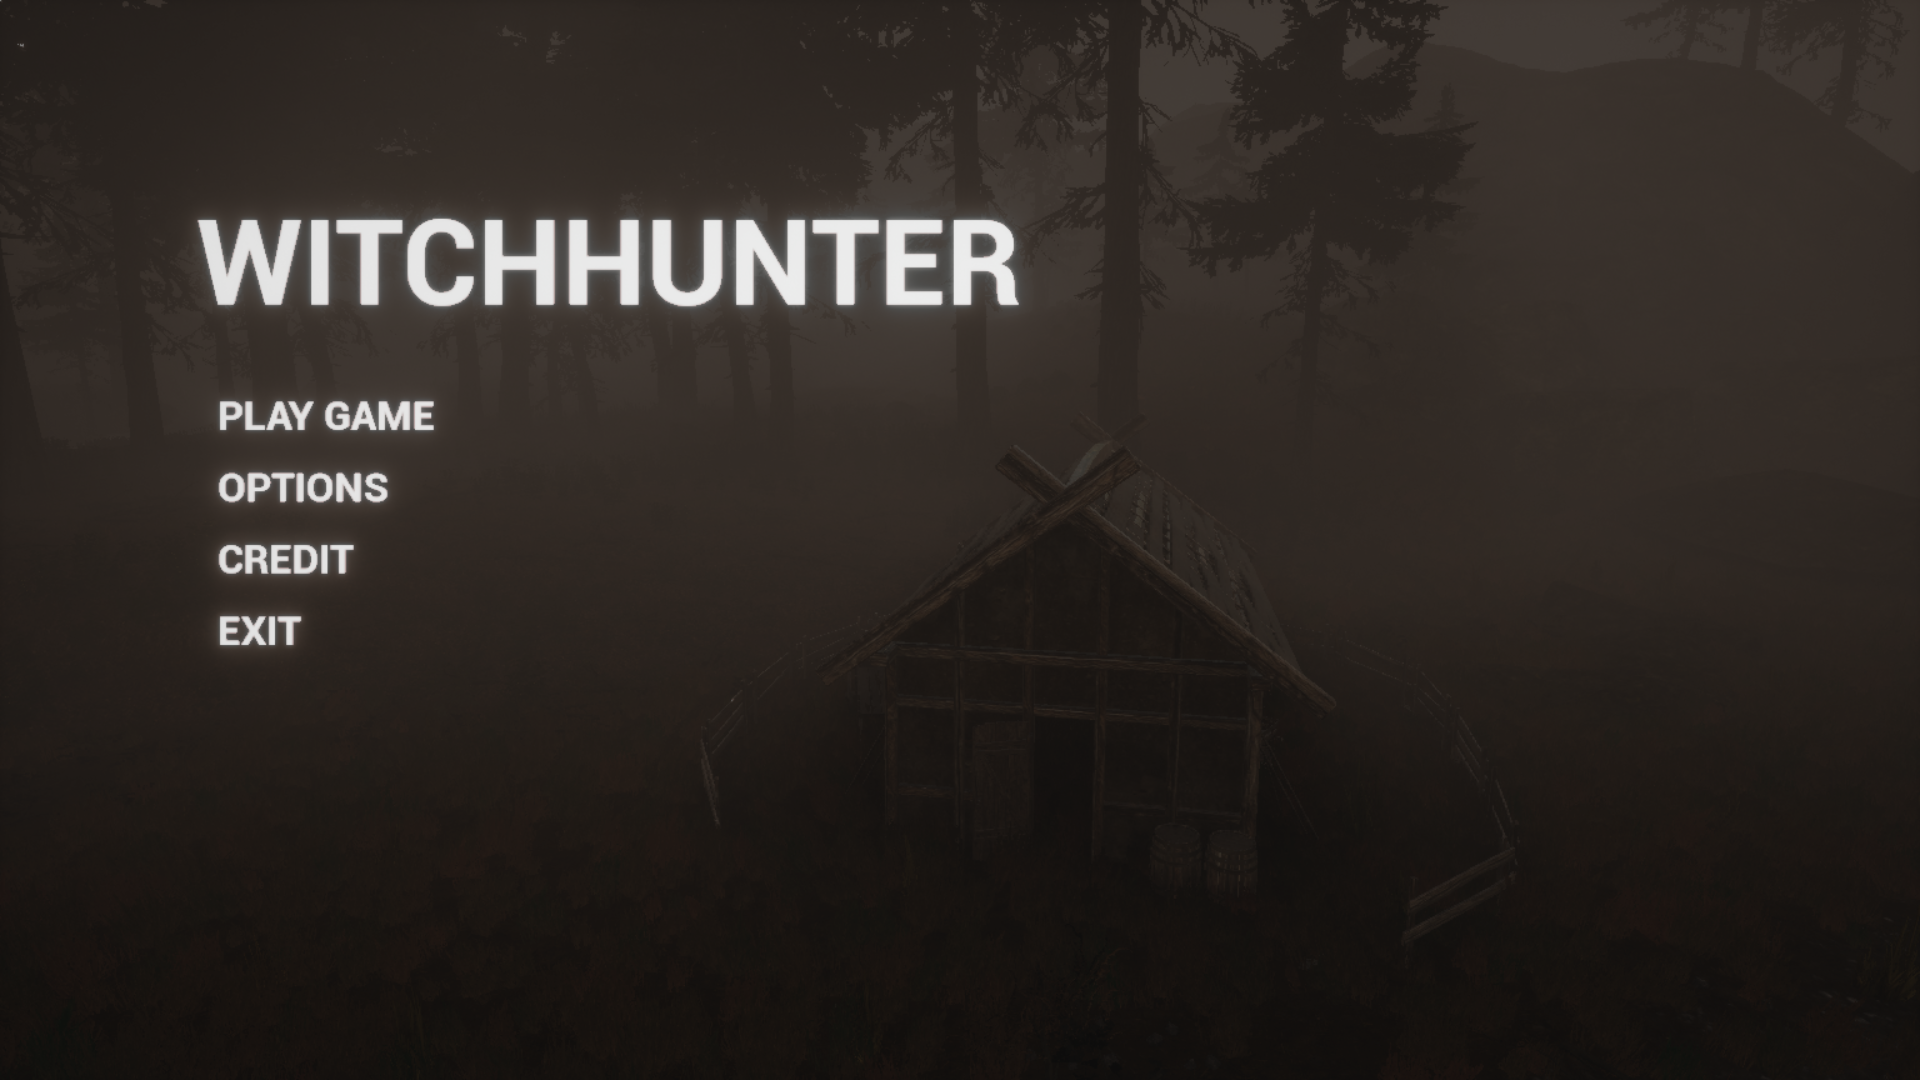
\includegraphics[width=\textwidth]{./img/UI/mainmenu.png}
  \end{center}
  \caption[หน้า Main Menu]{หน้า Main Menu}
  \label{fig:main_menu}
\end{figure}

\pagebreak

\begin{figure}[h!]
  \begin{center}
  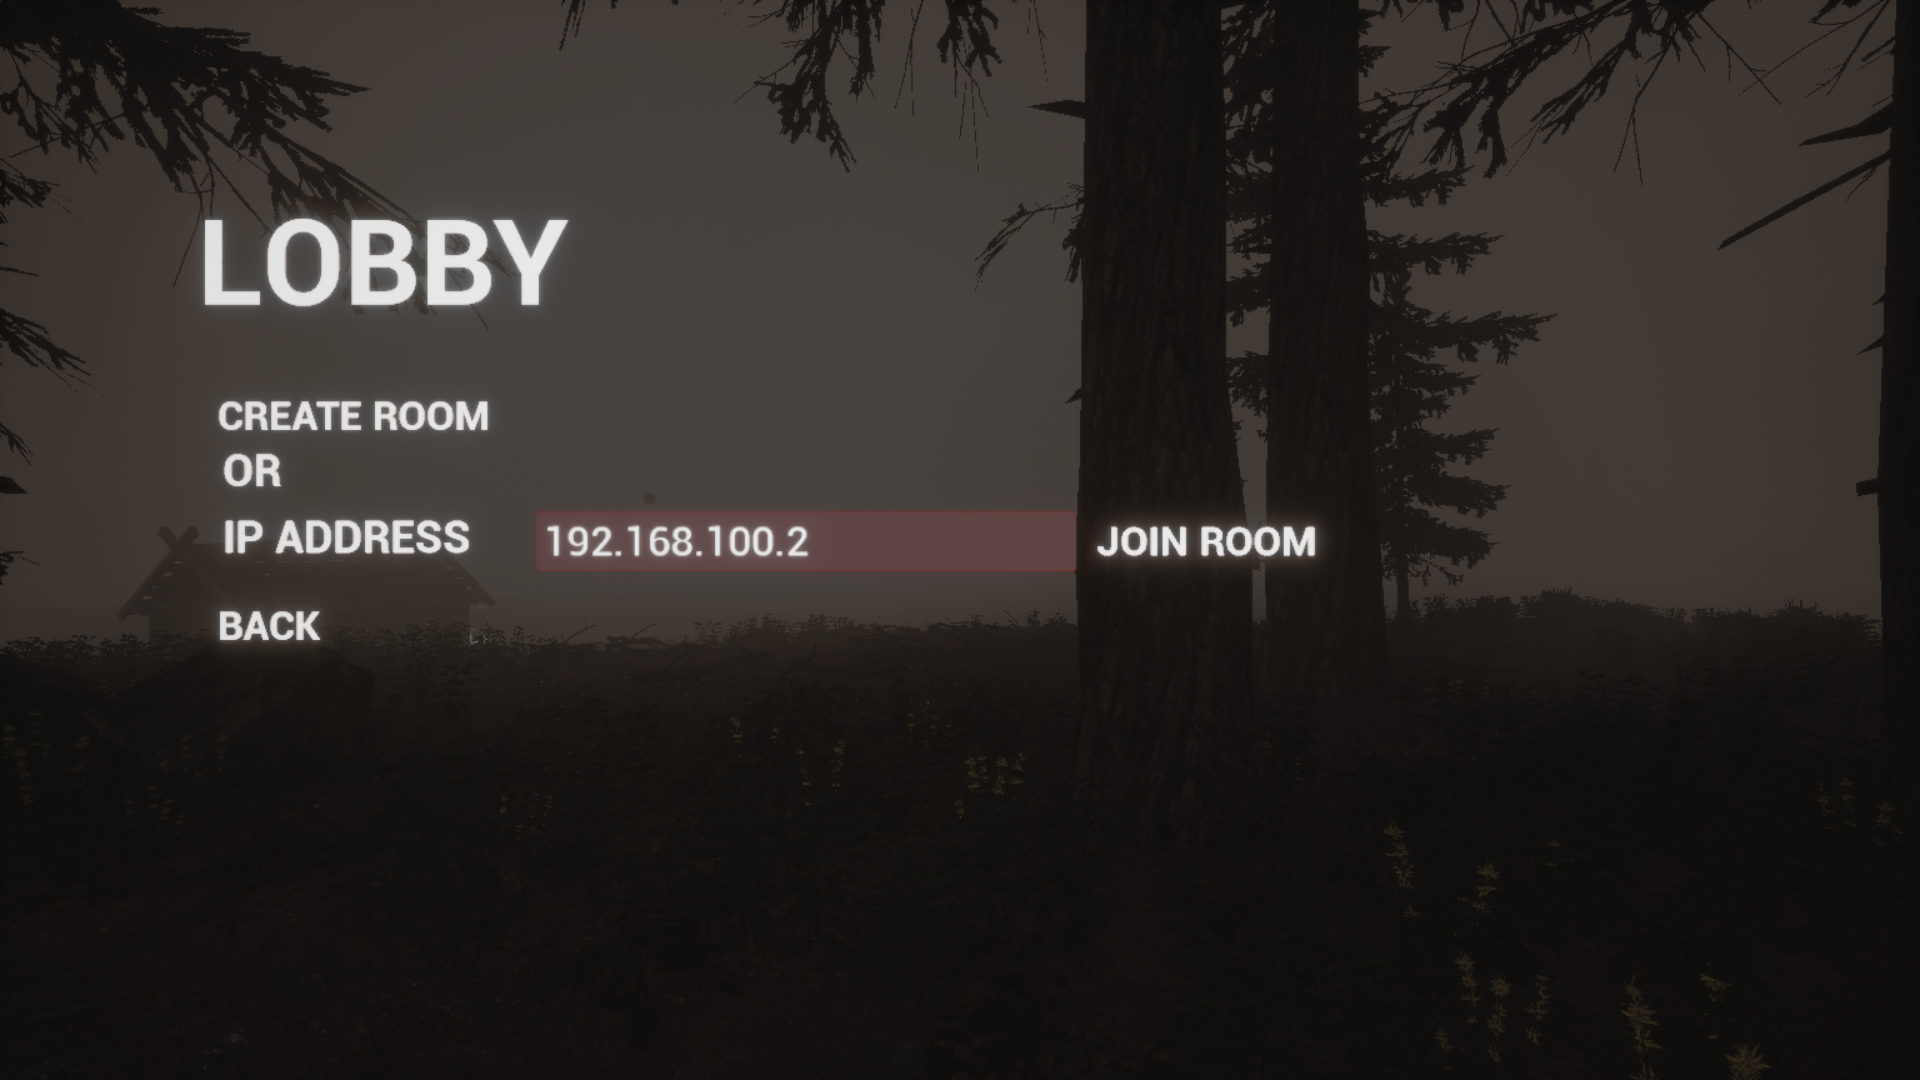
\includegraphics[width=\textwidth]{./img/UI/create_room.png}
  \end{center}
  \caption[หน้าสร้างห้องหรือเข้าร่วมห้อง]{หน้าสร้างห้องหรือเข้าร่วมห้อง}
  \label{fig:create_room}
\end{figure}

\begin{figure}[h!]
  \begin{center}
  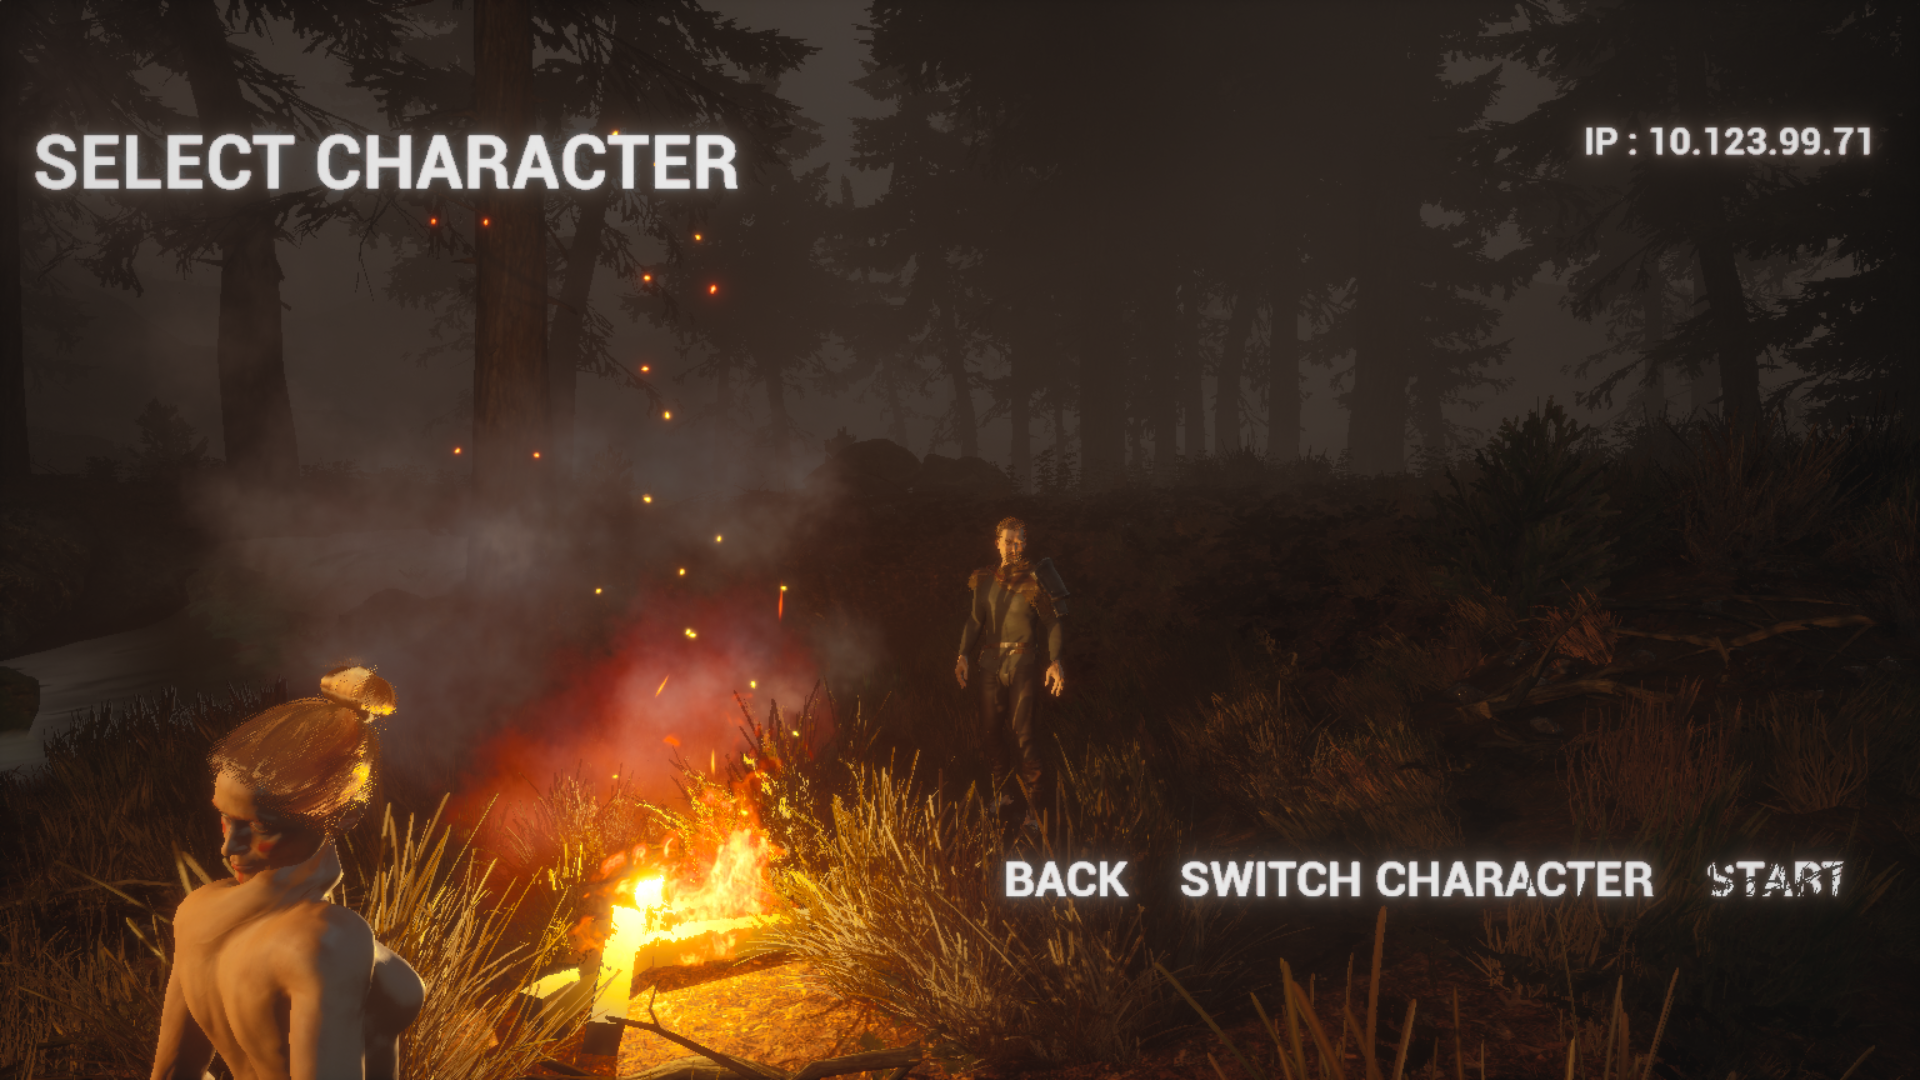
\includegraphics[width=\textwidth]{./img/UI/select_character.png}
  \end{center}
  \caption[หน้าเลือกตัวละครหลังจากเข้าร่วมห้องแล้ว]{ผู้เล่นสามารถเลือกฝ่ายและตัวละครที่อยากเล่นได้ด้วยการกดปุ่ม Switch Character และสามารถเห็นตัวละครของผู้เล่นคนอื่น ๆ}
  \label{fig:select_character}
\end{figure}

\subsubsection{UI ของฝ่าย Hunters}

ด้านบนซ้ายแสดงสถานะของเกม หลอด Circular Progress Bar แสดงเวลาในการทำภารกิจที่ยังเหลืออยู่ ถัดมาบอกจำนวนครั้งของพิธีที่ได้ทำไปแล้ว
ด้านล่างซ้ายแสดงเมนู Inventory

\begin{figure}[h]
  \begin{center}
  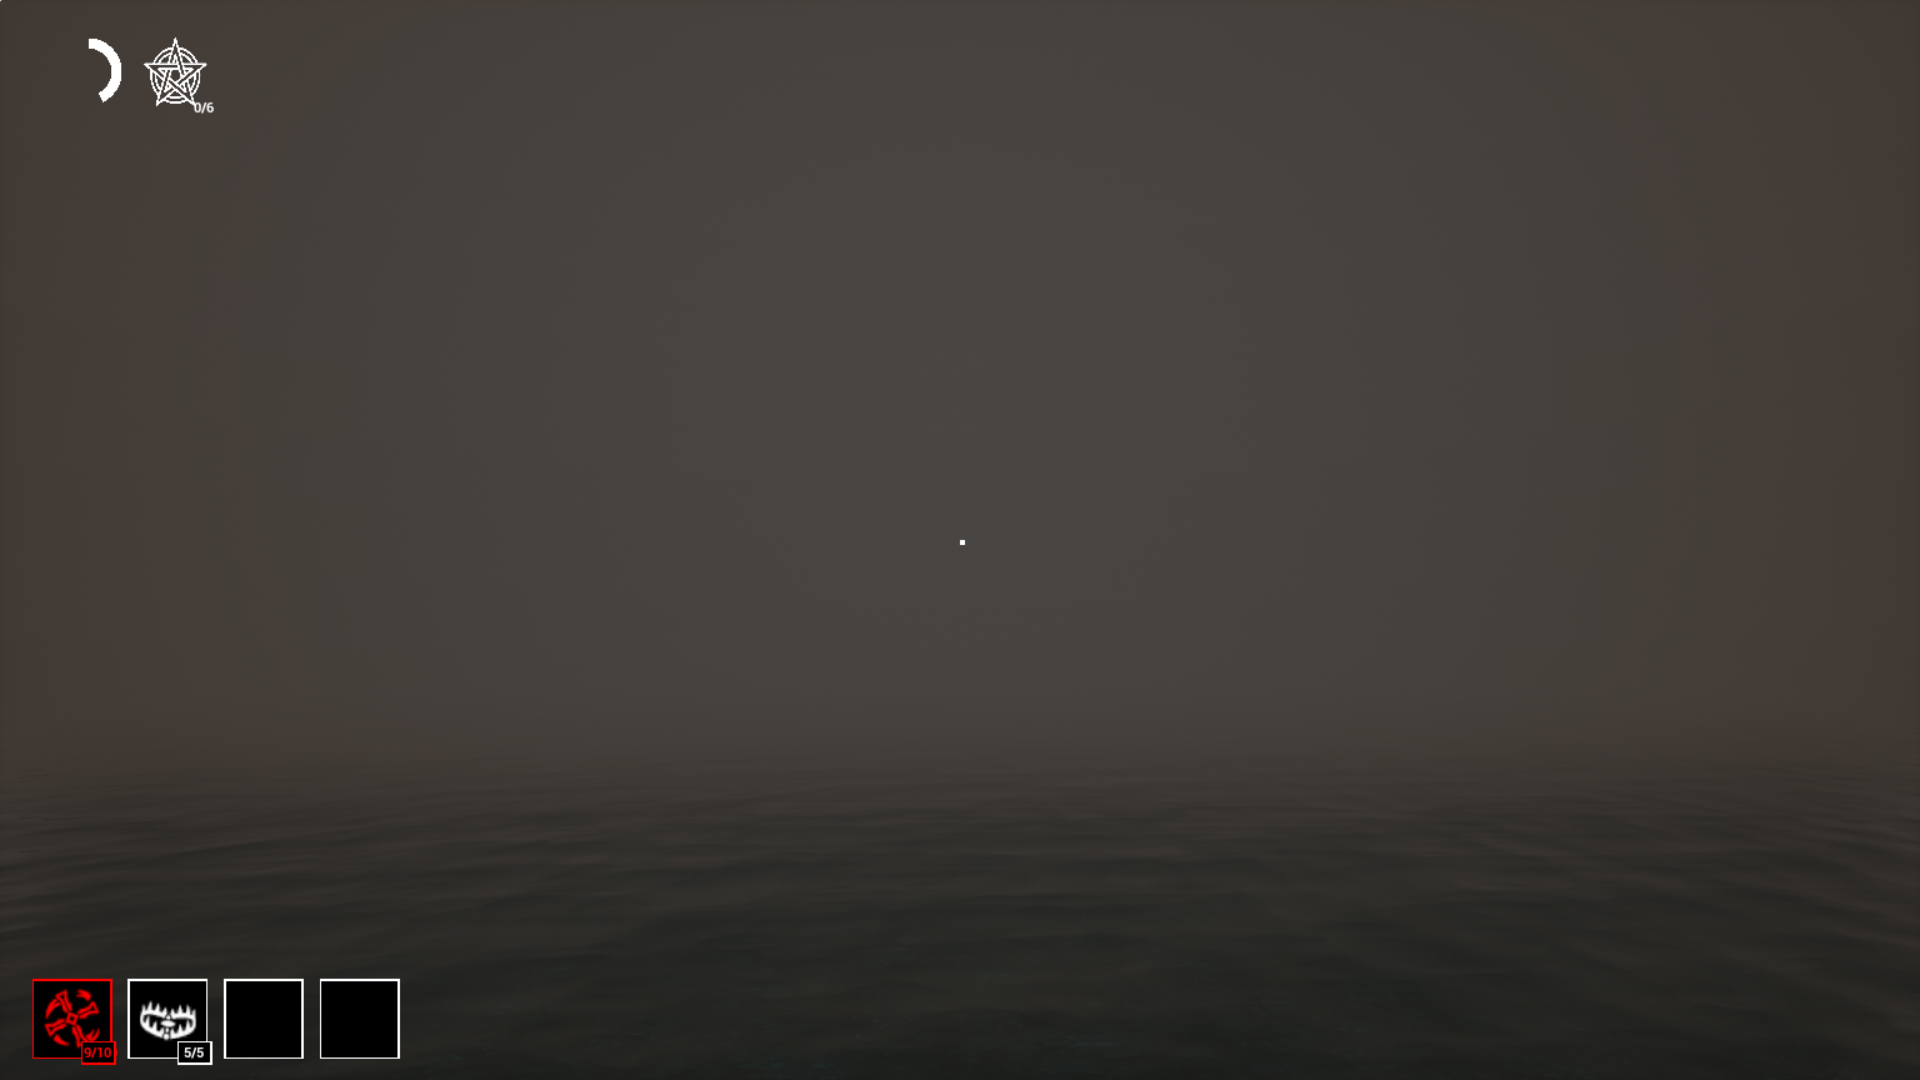
\includegraphics[width=0.8\textwidth]{./img/UI/hunter_ui.png}
  \end{center}
  \caption[ภาพ User Interface ของ Hunter]{ภาพ User Interface ของ Hunter}
  \label{fig:hunter_ui}
\end{figure}

\subsubsection{UI ของฝ่าย Witch}

ด้านบนซ้ายแสดงสถานะของเหมือนกับของ Hunter ด้านล่างซ้ายแสดงสถานะของความสามารถพิเศษที่สามารถสิงกวางได้ บอกถึงคูลดาวน์ของพลัง

\begin{figure}[h]
  \begin{center}
  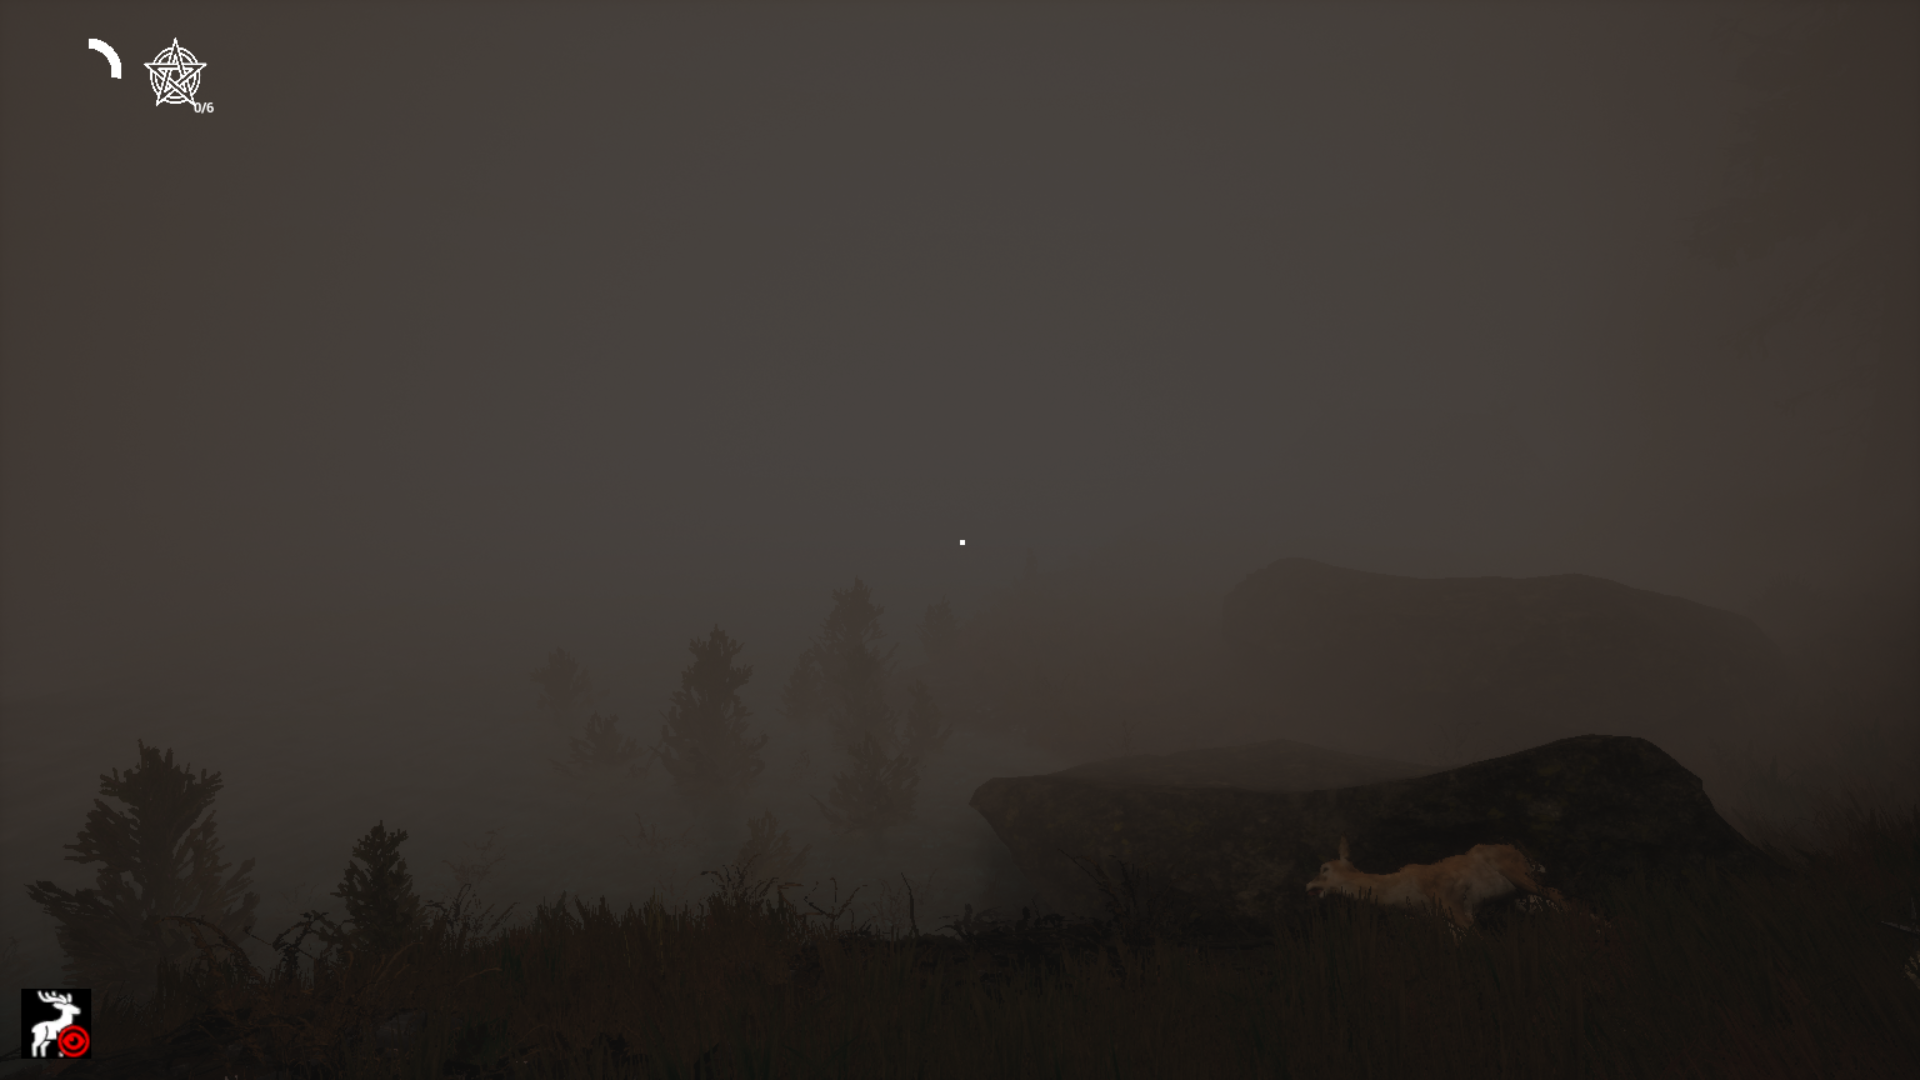
\includegraphics[width=0.8\textwidth]{./img/UI/witch_ui.png}
  \end{center}
  \caption[ภาพ User Interface ของ Witch]{ภาพ User Interface ของ Witch}
  \label{fig:witch_ui}
\end{figure}